
\chapter{METHODOLOGY}
{\baselineskip=2\baselineskip
This chapter discusses the research design and methodology employed in the study. It outlines the procedures for developing, implementing, and evaluating the multi-camera customer tracking system.

\section{Research Design and Procedure}
The study employed an experimental research design, incorporating multiple techniques across various phases to develop and evaluate the proposed system.

\begin{figure}[H]
	\caption[Modified Waterfall Model]{\newline \newline Modified Waterfall Model}
	\centering
	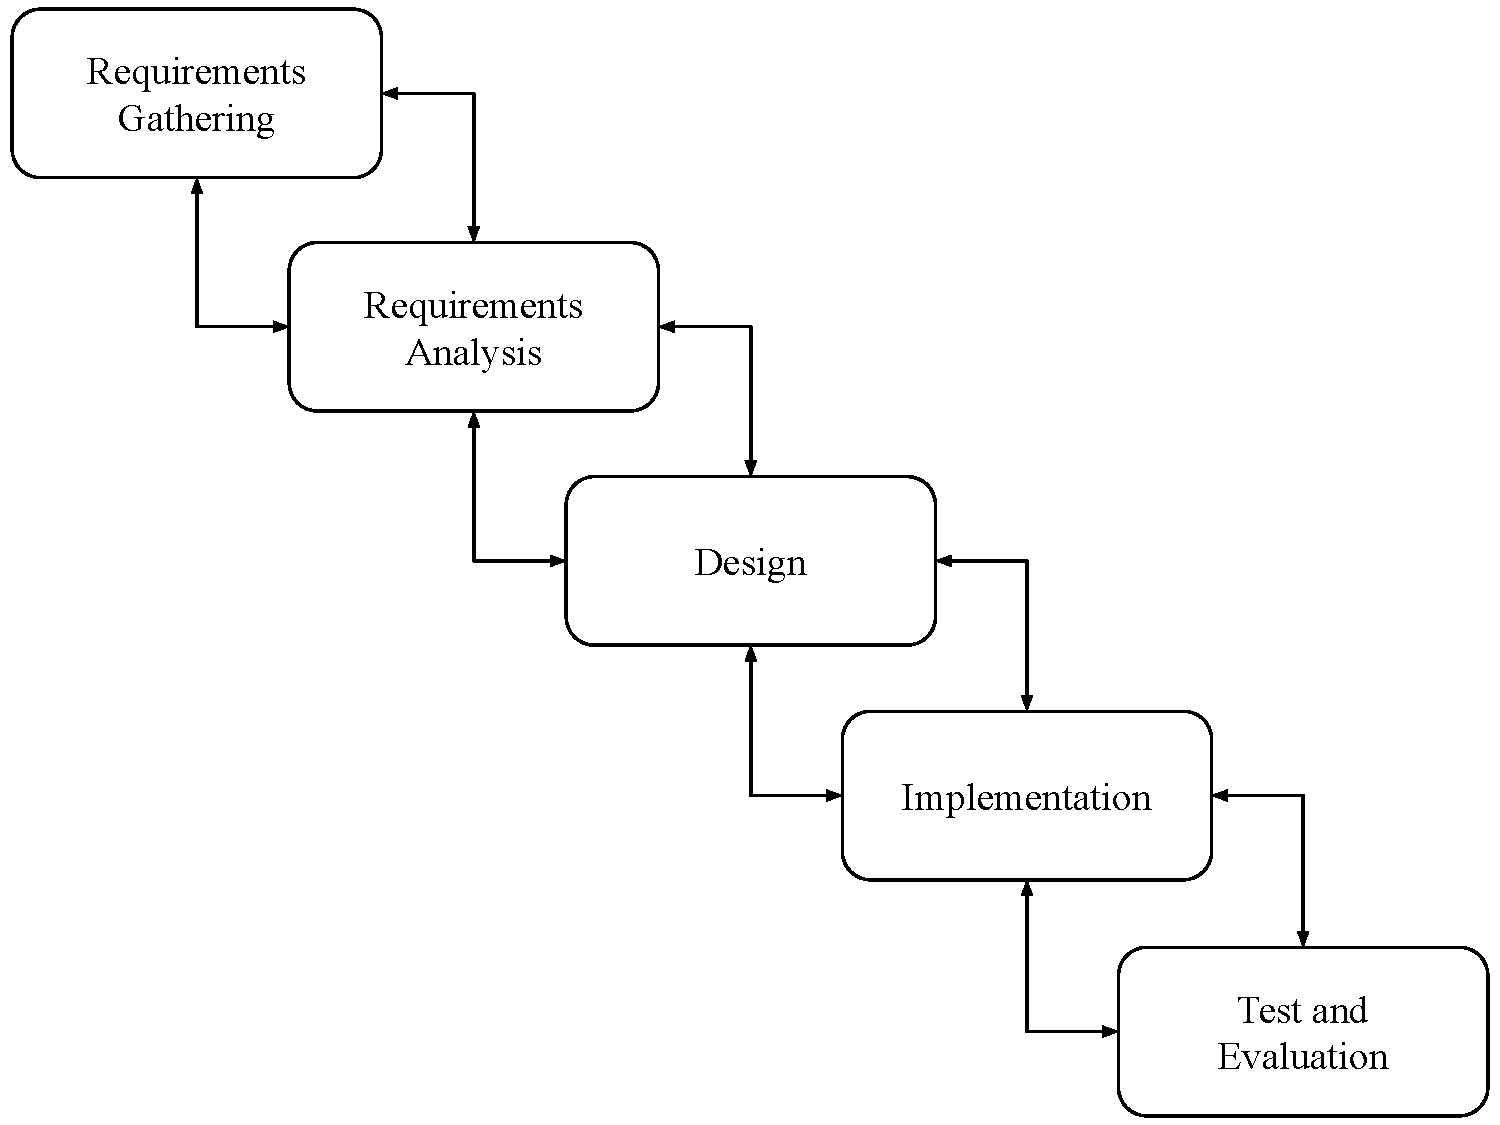
\includegraphics[width=0.7\linewidth]{fig/3.1.pdf}
	\label{fig:3.1}
\end{figure}
This approach enabled systematic testing and refinement through cycles of design, implementation, and assessment. To guide the development process, the researchers adopted a modified Waterfall Model from the System Development Life Cycle (SDLC).

Figure~\ref{fig:3.1} provides a structured framework, promoting a step-by-step progression from requirements gathering to evaluation while allowing for iterative improvements at each stage. The System Design section presents a more detailed discussion of the Modified Waterfall Model, including its phases and adaptations for the study.

\section{Research Setting}

\begin{figure}[H]
	\caption[The Retail Shop in Market City, Agora, Lapasan]{\newline \newline The Retail Shop in Market City, Agora, Lapasan}
	\centering
	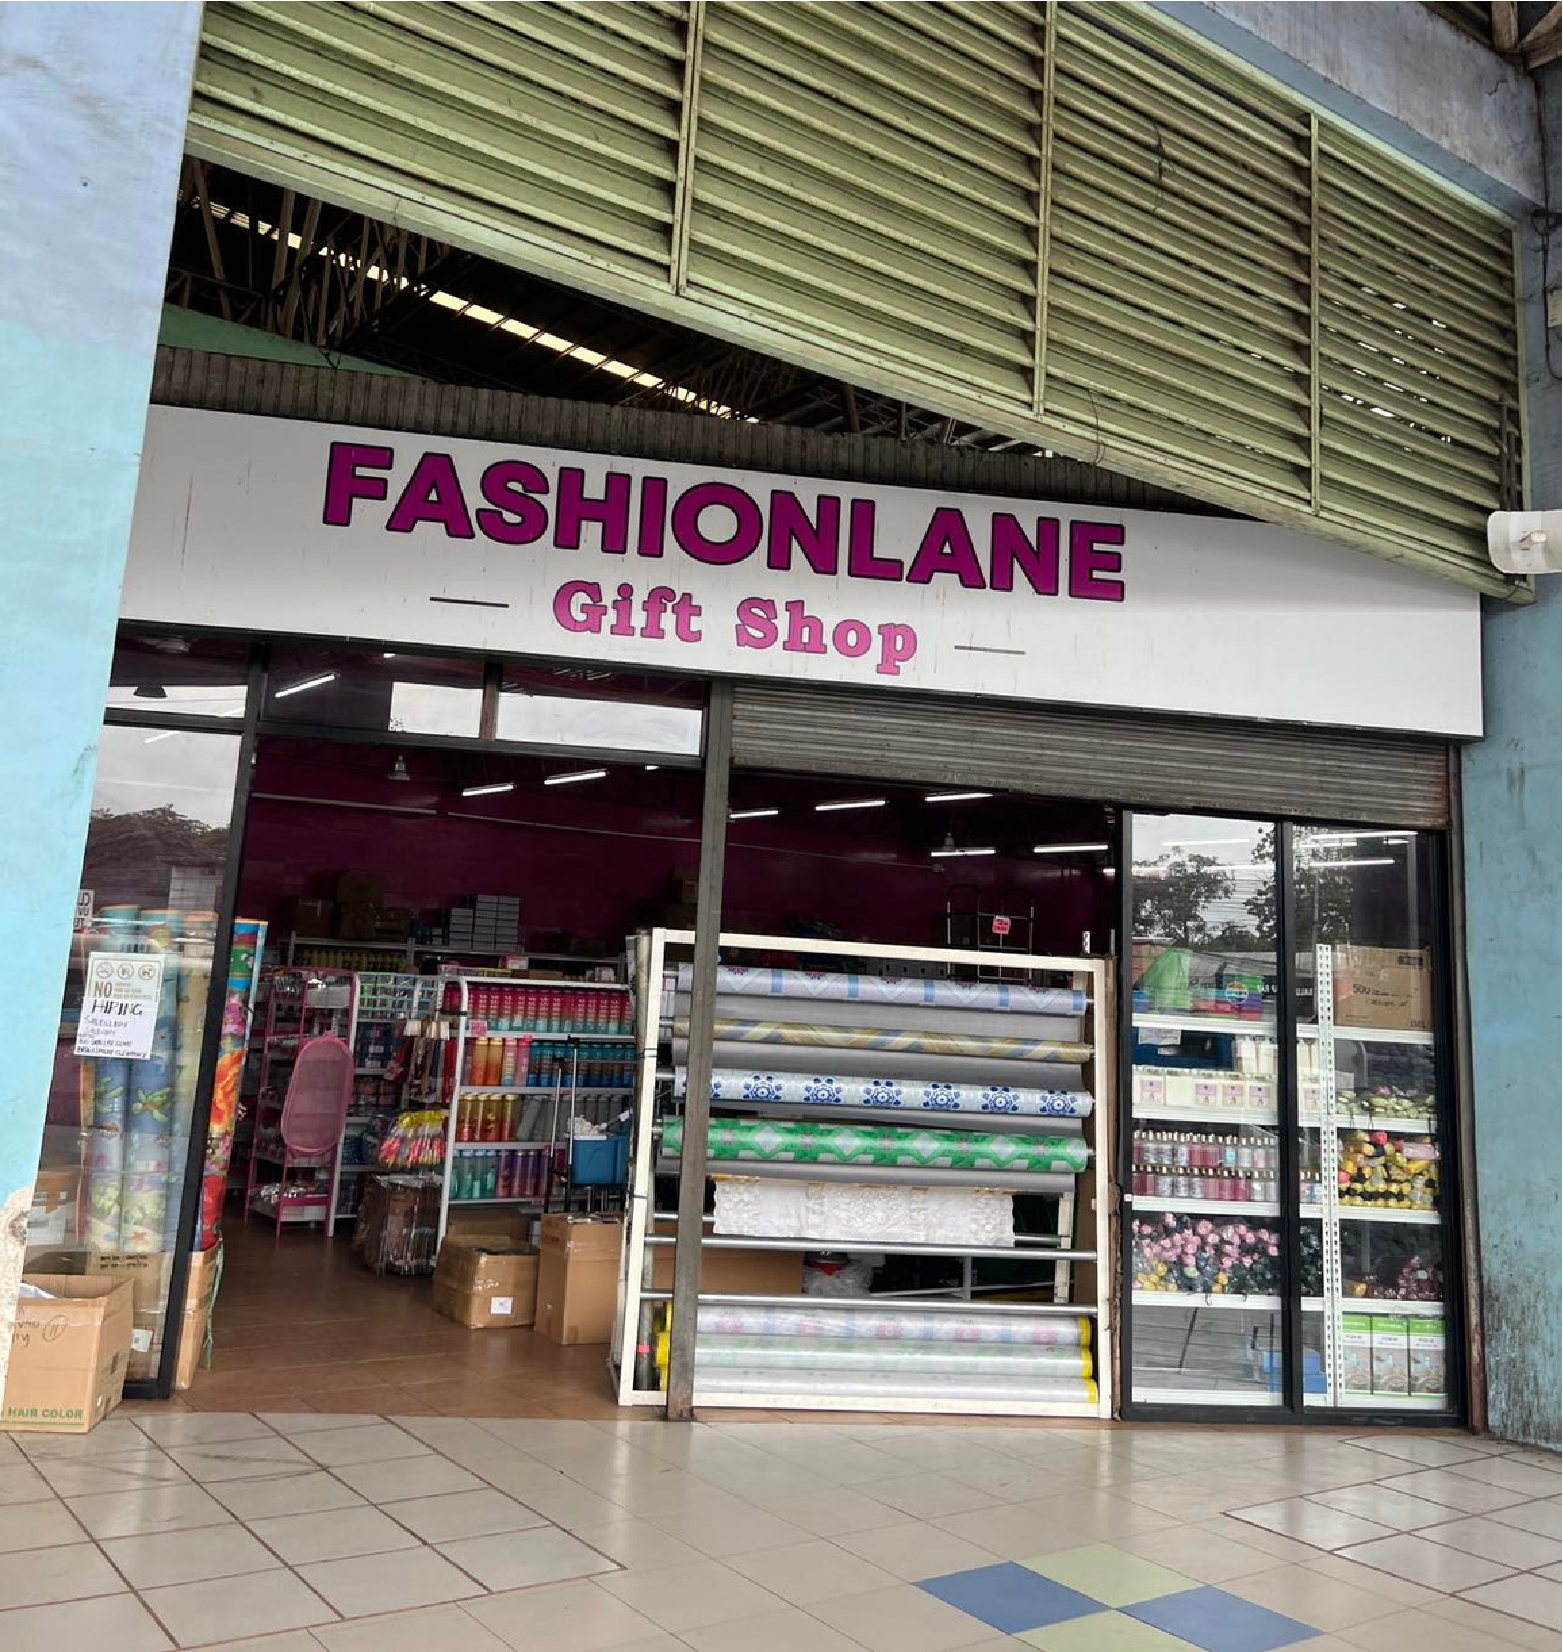
\includegraphics[width=0.5\linewidth]{fig/3.2.pdf}
	\label{figs:3.2}
\end{figure}

The study was conducted at a gift shop located in Market City, Agora, Lapasan, Cagayan de Oro City, shown in Figure~\ref{figs:3.2}. Although the original proposal considered a general merchandise store, the researchers pivoted to the gift shop after assessing its suitability. Despite the change, the store still qualifies as a retail environment, offering a wide range of consumer goods, including body and bath products, cosmetics, school supplies, kitchenware, and home items. Customers freely browse and interact with these products, making it ideal for behavioral observation.

The shop was chosen not only for its product diversity and retail nature but also for its existing CCTV surveillance system, which met the system’s technical requirements. The structured store layout with clear aisles and zones allowed the researchers to define Regions of Interest (ROIs) for tracking movement and behavior. Camera placement covered essential areas like entrances and display zones, requiring only minimal adjustments. Additionally, the store’s location within a busy terminal ensured consistent customer traffic, which was vital for collecting meaningful behavior data. These factors made the gift shop a practical and effective setting for implementing and evaluating the SUBAY system.

\section{Research Setup}

The research setup utilized four existing closed-circuit television (CCTV) cameras from the selected retail environment to ensure comprehensive coverage of key areas. These cameras were strategically positioned to monitor high-traffic zones such as entrances, aisles, and product displays, supporting the requirements of the multi-camera tracking system. Since the surveillance infrastructure was already in place, no additional hardware installation was necessary. Each camera provided a distinct perspective, enabling seamless tracking of customer movement across different sections of the store. Their reliability and high-definition video quality ensured clear footage essential for testing and evaluation.

\begin{figure}[H]
	\caption[Chosen Camera Views Inside the Gift Shop]{\newline \newline Chosen Camera Views Inside the Gift Shop}
	\centering
	\includegraphics[width=1\linewidth]{fig/3.3.pdf}
	\label{fig:3.3}
\end{figure}

Figure~\ref{fig:3.3} presents the selected overlapping camera views (Camera 02, 03, 05, and 09), each strategically chosen for optimal aisle zone visibility, including AISLE 1 through AISLE 6. The layout spans a total distance of 21 meters, with Camera 03 positioned approximately 21 meters from the main aisle area, covering the front desk entrance to minimize obstructions and avoid heavy backlighting. Camera 02 monitors AISLE 1 and AISLE 2, providing visibility of customer movement and interactions near the entrance. Camera 05 covers AISLE 3 and AISLE 4, ensuring high-resolution imaging for accurate detection, while Camera 09 captures AISLE 5 and AISLE 6, completing the surveillance coverage and enhancing overall detection accuracy. The placements were carefully designed to reduce blind spots, maintain image clarity, and optimize performance in varying lighting conditions.

\section{System Design}

This section details the system development process based on the modified Waterfall Model from the System Development Life Cycle (SDLC). It outlines the major phases followed in building the multi-camera customer tracking system, including requirements gathering, analysis, design, implementation, and testing and evaluation.

\subsection{Requirements Gathering}
The requirements gathering process was conducted through an in-person visit and interview with the retail store owner, selected as the primary respondent due to their familiarity with store operations, surveillance practices, and customer behavior. The main objective was to collect essential information for system development and to request formal permission to access the store’s existing CCTV footage.

Before the engagement, the researchers prepared a set of open- and closed-ended questions to guide the discussion, focusing on customer flow, surveillance coverage, and the general store layout. A consent letter outlining the ethical use of the collected data was presented, ensuring that footage and behavioral information would be used solely for academic and research purposes in compliance with data privacy regulations. The store owner reviewed and approved the terms, granting permission to access the CCTV system under agreed conditions.

The interview, conducted on-site with the respondent’s consent, provided insights into camera placements, zones of customer interest, existing challenges in tracking behavior, and the store’s goals for analyzing foot traffic and customer interaction with displays. Complementing the interview, the researchers also conducted field observations, noting customer movement patterns, entry points, checkout counters, and high-interest product areas. The CCTV system was assessed for its coverage, resolution, and timestamp synchronization, all crucial for supporting the proposed tracking and analytics features.

One key insight was the store owner's difficulty in manually interpreting customer activity from raw footage and their interest in an automated solution for analyzing foot traffic and generating behavioral reports. These findings helped define the system’s requirements, ensuring ethical data use while addressing operational needs and aligning with real-world store conditions.

\subsection{Requirements Analysis}
After the requirements gathering process, the researchers compiled and analyzed the data collected from interviews and on-site observations at the retail store. This process enabled them to understand the store’s operational needs, the technological environment, particularly the existing CCTV infrastructure, and the store owner's expectations regarding customer behavior insights.

To support the system’s development and ensure the accuracy of data collection, the researchers were granted secure access to the store's CCTV Video Management Software: iVMS-4200 and Hik-Connect. Access to login credentials and video footage was provided strictly for this study, and all data handling was conducted with strict adherence to privacy protection and confidentiality protocols.

Based on the analysis, the researchers identified the system’s primary users: the Customers and the Retail Store Owner or Manager. While customers are not direct users of the system interface, their behavior and interactions within the store serve as the primary input for the system’s analytical processes. In contrast, the Retail Store Owner or Manager is the principal system user, utilizing the dashboard and generated reports to make informed decisions on store layout and marketing strategies.

\subsubsection{User Definition}

Following the requirements analysis, the system's users were defined as follows:

\textbf{Customers} - Customers are the subjects of data collection. Their movements and interactions within the store are passively monitored through the CCTV infrastructure to generate behavioral analytics.

\textbf{Retail Store Owner/Manager} - The system’s primary user accesses the dashboard, retrieves behavioral reports, and uses the insights generated to optimize store layout and develop marketing strategies.

The specific user requirements are summarized in Table 3.1.

{\setstretch{1.5}
	\begin{longtable}{|p{4cm}|p{11cm}|}
		\caption[User Requirements Table]{\newline \newline User Requirements Table} \label{tab:user-requirements} \\
		\hline
		\textbf{User} & \textbf{Requirement} \\
		\hline
		\endfirsthead
		
		\multicolumn{2}{c}{Table \thetable{} -- continued from previous page} \\
		\hline
		\textbf{User} & \textbf{Requirement} \\
		\hline
		\endhead
		
		\hline \multicolumn{2}{r}{Continued on next page} \\
		\endfoot
		
		\hline
		\endlastfoot
		
		Customer (Indirect) & 
		- Their presence and behavior must be passively and anonymously tracked. \newline
		- Their data must be handled ethically and used solely for research purposes. \\
		\hline
		Retail Store Owner/Manager &
		- Access to a visual dashboard summarizing customer movement and behaviors. \newline
		- Ability to retrieve and download behavioral analytics reports. \newline
		- Tools to analyze foot traffic patterns and product interaction frequency. \newline
		- Insights to support decision-making for store layout and marketing strategies. \newline
		- Ensure that the system does not compromise customer privacy. \\
		\hline
	\end{longtable}
}

This analysis laid the foundation for defining the system’s core features and ensuring that development aligned with both operational needs and ethical considerations.

\subsubsection{System Requirements}
The system requirements, shown in Table~\ref{tab:system-requirements}, were categorized into Input, Process, Output, Control, and Performance specifications to guide system design and implementation.

{\setstretch{1.25}
\begin{longtable}{|p{4cm}|p{11cm}|}
		\caption[System Requirements]{\newline \newline System Requirements Table} \label{tab:system-requirements} \\
		\hline
		\textbf{Category} & \textbf{System Requirement} \\
		\hline
		\endfirsthead
		
		\multicolumn{2}{l}{\tablename\ \thetable{} -- \textit{continued from previous page}} \\
		\hline
		\textbf{Category} & \textbf{System Requirement} \\
		\hline
		\endhead
		
		\hline \multicolumn{2}{|r|}{{Continued on next page}} \\ \hline
		\endfoot
		
		\hline
		\endlastfoot
		
		Input Requirements & 
		- The system shall accept video feeds from the store's existing CCTV infrastructure. \newline
		- The system shall detect and track customer presence in and upon entering the store. \newline
		- The system shall capture customer movement across different store zones. \newline
		- The system shall detect customer visits and dwell time in zones. \newline
		- The system shall log entry/exit points and dwell times automatically. \\*
		\hline
		Process Requirements & 
		- The system shall use object detection (YOLO) and tracking algorithms (DeepSORT) to assign customers unique tracking IDs. \newline
		- The system shall process and analyze customer movement patterns throughout the store. \newline
		- The system shall compile and aggregate behavioral data for further analysis. \newline
		- The system shall anonymize customer data to ensure privacy during processing. \newline
		- The system shall store processed behavioral data in a secure database for future retrieval. \newline
		- The system shall link zone-specific behaviors to product interaction and foot traffic trends. \\
		\hline
		
		Output Requirements & 
		- The system shall display summarized analytics through a visual dashboard. \newline
		- The system shall generate and display foot traffic heat maps and trend charts. \newline
		- The system shall produce downloadable behavioral reports filtered by date range. \newline
		- The system shall show customer interaction metrics such as dwell time per product zone. \\
		\hline
		
		Control Requirements & 
		- The system must secure access through administrator login credentials and restrict sensitive data access to authorized personnel only. \newline
		- The system shall not collect personally identifiable information (PII) from customers (such as social security numbers, full names, email addresses, or phone numbers). \\
		\hline
		
		Performance Requirements & 
		- The system must ensure high accuracy in detecting and tracking customers even in crowded environments. \newline
		- The system shall be capable of handling multiple video feeds simultaneously. \newline
		- The system shall ensure the responsive performance of the dashboard interface and analytics tools. \\
		\hline
		
\end{longtable}
}

The system requirements were developed based on the data collected during the requirements gathering phase. The primary objective of the system is to leverage the store’s existing CCTV infrastructure to anonymously track customer movement and interactions and generate actionable behavioral analytics for the retail store owner. Input requirements focus on collecting movement and interaction data, which are processed using AI-based object detection and tracking algorithms while ensuring customer anonymity. Outputs are presented through an interactive dashboard that provides insights such as foot traffic heat maps, aisle visitation metrics, and customer behavior trends. Control measures guarantee that privacy and data protection standards are strictly observed, while performance requirements ensure the system operates efficiently, accurately, and reliably to support business decision-making.

\subsection{Design}
This section presents the system's design. The researchers worked on a design that would meet the specifications described in the system requirements. To illustrate the system's design, context-level diagrams, data flow diagrams, use case diagrams, activity diagrams, and system architecture were used.

\subsubsection{Context-Level Diagram}
The Context-Level Diagram provides a high-level view of how the SUBAY system interacts with its primary stakeholders: Customers and Retail Store Owners/Managers. It illustrates how data flows into and out of the system without detailing internal processes.

Figure~\ref{fig:3.4} presents the interaction between Customers and the SUBAY system from the perspective of behavioral input and experiential output. While customers do not directly interact with the system, their natural behaviors, such as walking through aisles, pausing at displays, and engaging with products, serve as critical input for SUBAY’s analytics. 

\begin{figure}[H]
	\caption[Context-Level Diagram for Customers]{\newline \newline Context-Level Diagram for Customers}
	\centering
	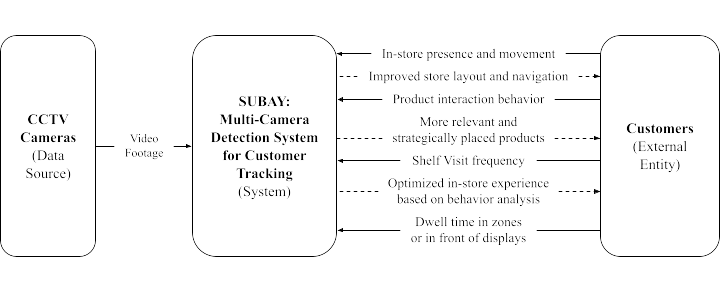
\includegraphics[width=1\linewidth]{fig/3.4.pdf}
	\label{fig:3.4}
\end{figure}

These activities are continuously captured by the existing CCTV infrastructure and analyzed using object detection and multi-camera tracking technologies. The system interprets these behavioral inputs to generate key metrics, including dwell times, zone engagements, visit frequencies, and interaction hotspots. 

\begin{figure}[H]
	\caption[Context-Level Diagram for Retail Store Owners/Managers]{\newline \newline Context-Level Diagram for Retail Store Owners/Managers}
	\centering
	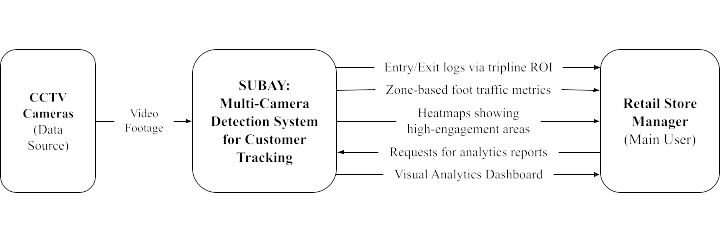
\includegraphics[width=1\linewidth]{fig/3.5.pdf}
	\label{fig:3.5}
\end{figure}

Figure~\ref{fig:3.5} illustrates the system’s interaction with Retail Store Owners and Managers. CCTV cameras are the primary data source, capturing continuous video streams throughout the store. The SUBAY system processes these video feeds to extract actionable insights. The system outputs include entry and exit logs based on tripline detection, zone-based foot traffic analytics, and heat maps highlighting customer engagement patterns. Through a visual analytics dashboard, store owners and managers access metrics, generate customized reports, and make informed decisions about store layouts and marketing initiatives. This context-level view highlights the end-to-end data flow, from passive customer behavior captured on video to strategic insights that empower retail decision-making.

\subsubsection{Data Flow Diagram}

The Data Flow Diagram (DFD) provides a detailed view of how information moves through the SUBAY system, highlighting the key processes that transform raw data into actionable insights for end-users.

\begin{figure}[H]
	\caption[Data Flow Diagram for Customers]{\newline \newline Data Flow Diagram for Customers}
	\centering
	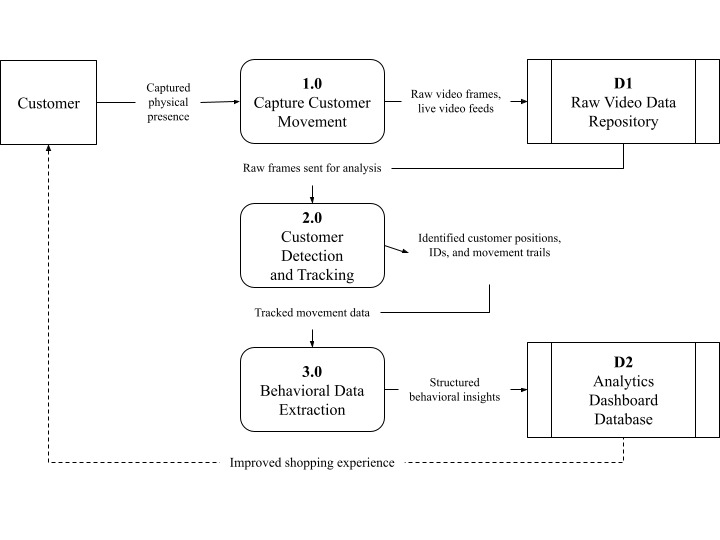
\includegraphics[width=0.80\linewidth]{fig/3.6.pdf}
	\label{fig:3.6}
\end{figure}

\vspace{1em}

Figure~\ref{fig:3.6} illustrates how customer movement within the retail environment initiates the system’s data flow. Without direct input from customers, their presence and actions are captured through continuous video streams. In Process 1.0, these streams are received and prepared for analysis. Process 2.0 applies object detection and multi-camera tracking algorithms to extract movement patterns, paths, and interaction points. The processed movement data is then structured and organized in Process 3.0 before being stored securely in Data Store D2. Although customers remain unaware of these technical operations, the resulting insights significantly improve their shopping experience.

\begin{figure}[H]
	\caption[Data Flow Diagram for Retail Store Owners/Managers]{\newline \newline Data Flow Diagram for Retail Store Owners/Managers}
	\centering
	
\includegraphics[width=1\linewidth]{fig/3.7.pdf}
	\label{fig:3.7}
\end{figure}

Figure~\ref{fig:3.7} presents the Level 1 Data Flow Diagram focused on Retail Store Owners and Managers. The system processes the structured behavioral datasets collected from detection and tracking outputs in Process 1.0 to generate analytical summaries. These summaries are stored in Data Store D1 for retrieval. In Process 2.0, the stored analytics are accessed, organized, and prepared for visualization. Finally, Process 3.0 transforms the data into user-friendly charts, reports, and trend analyses, such as aisles with peak traffic, aisle-specific dwell times, foot traffic charts. Retail store owners access these insights via the dashboard, enabling them to make data-driven decisions.

\subsubsection{Use Case Diagram}
The Use Case Diagram visually represents how different actors interact with the SUBAY system. It captures passive and active engagements that drive data collection and system usage.

\begin{figure}[H]
	\caption[Use Case Diagram for Customers]{\newline \newline Use Case Diagram for Customers}
	\centering
	
\includegraphics[width=0.50\linewidth]{fig/3.8.pdf}
	\label{fig:3.8}
\end{figure}

Figure~\ref{fig:3.8} depicts how shoppers interact indirectly with the retail environment enhanced by SUBAY’s multi-camera detection system. The process begins when a customer enters the store, triggering the initialization of tracking through strategically positioned cameras. As the customer moves across various store zones, the system’s object detection and tracking algorithms monitor and record their paths, dwell times, and interactions with product displays. These interactions are captured passively without disrupting the natural shopping experience. Data such as zone engagement and product interaction durations are aggregated. The insights generated from these behaviors inform store adjustments like layout optimization and targeted promotions.

\begin{figure}[H]
	\caption[Use Case Diagram for Retail Store Owners/Managers]{\newline \newline Use Case Diagram for Retail Store Owners/Managers}
	\centering
	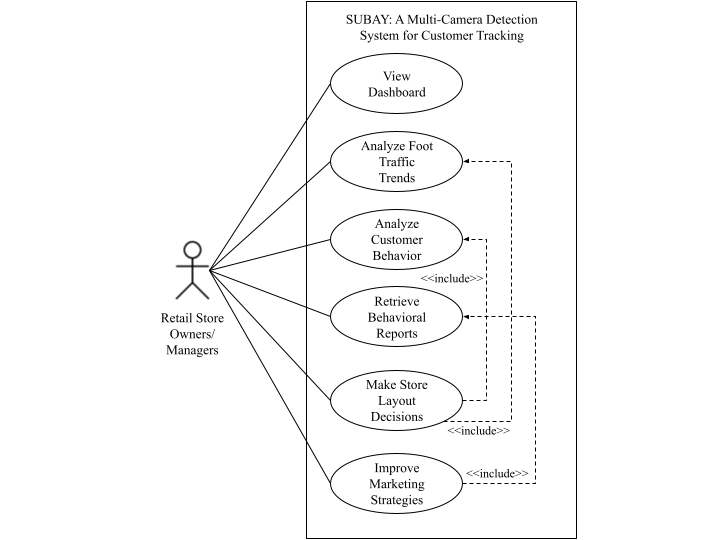
\includegraphics[width=1\linewidth]{fig/3.9.pdf}
	\label{fig:3.9}
\end{figure}

Figure~\ref{fig:3.9} illustrates the interaction between retail store owners or managers and the SUBAY system. Users can view the dashboard to access customer tracking insights. From this central interface, they can analyze zone-specific foot traffic and dwell time trends, which are included use cases essential for data-driven decision-making. These analytics support key business activities such as making store layout decisions and improving marketing strategies. Additionally, the system enables retrieval of detailed insight reports, helping managers better understand customer behavior. The use case relationships demonstrate how SUBAY streamlines customer analytics to help store owners optimize operations and enhance the overall shopping experience.

\subsubsection{Activity Diagram}

The Activity Diagram details the sequence of operations within the SUBAY system, highlighting the dynamic flow of actions between the system and its users.

\begin{figure}[H]
	\caption[Activity Diagram for Customers]{\newline \newline Activity Diagram for Customers}
	\centering
	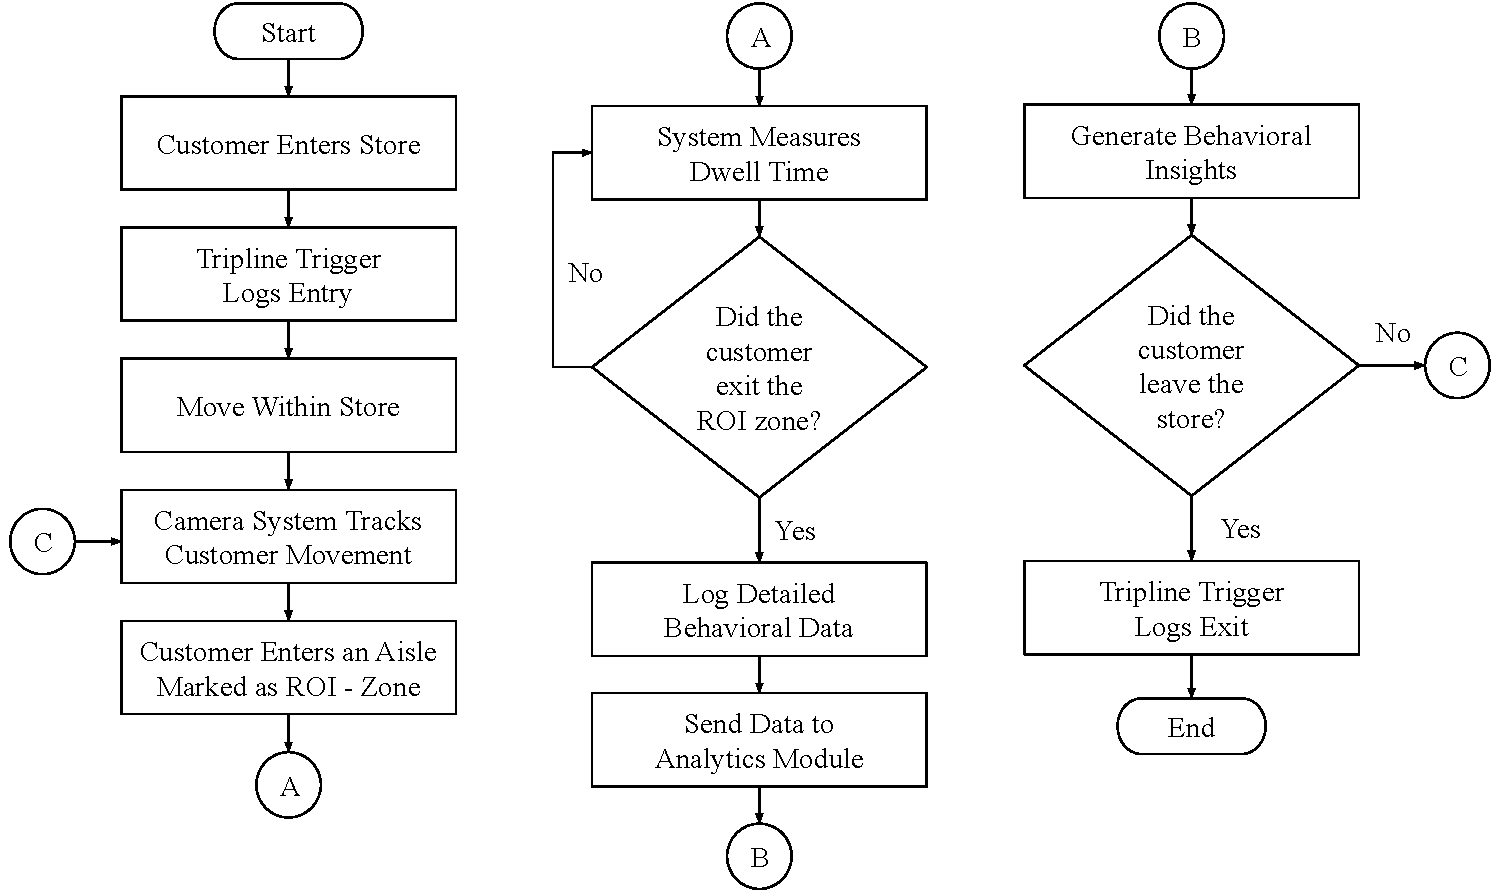
\includegraphics[width=0.75\linewidth]{fig/3.10.pdf}
	\label{fig:3.10}
\end{figure}

Figure~\ref{fig:3.10} illustrates the customer activity flow within the retail environment. The process begins when a customer enters the store, automatically triggering the customer-counting system, which logs their entry. As the customer navigates the store, the system passively monitors their movement. When customers enter a designated zone and interact with product displays, the system measures their dwell time. If the customer remains in the zone, dwell time is continuously recorded; otherwise, if they move out, the system logs the interaction and resumes tracking across other zones. Upon exiting the store, the system records their departure, closing the tracking session.

\begin{figure}[H]
	\caption[ Activity Diagram for Retail Store Owners/Managers]{\newline \newline Activity Diagram for Retail Store Owners/Managers}
	\centering
	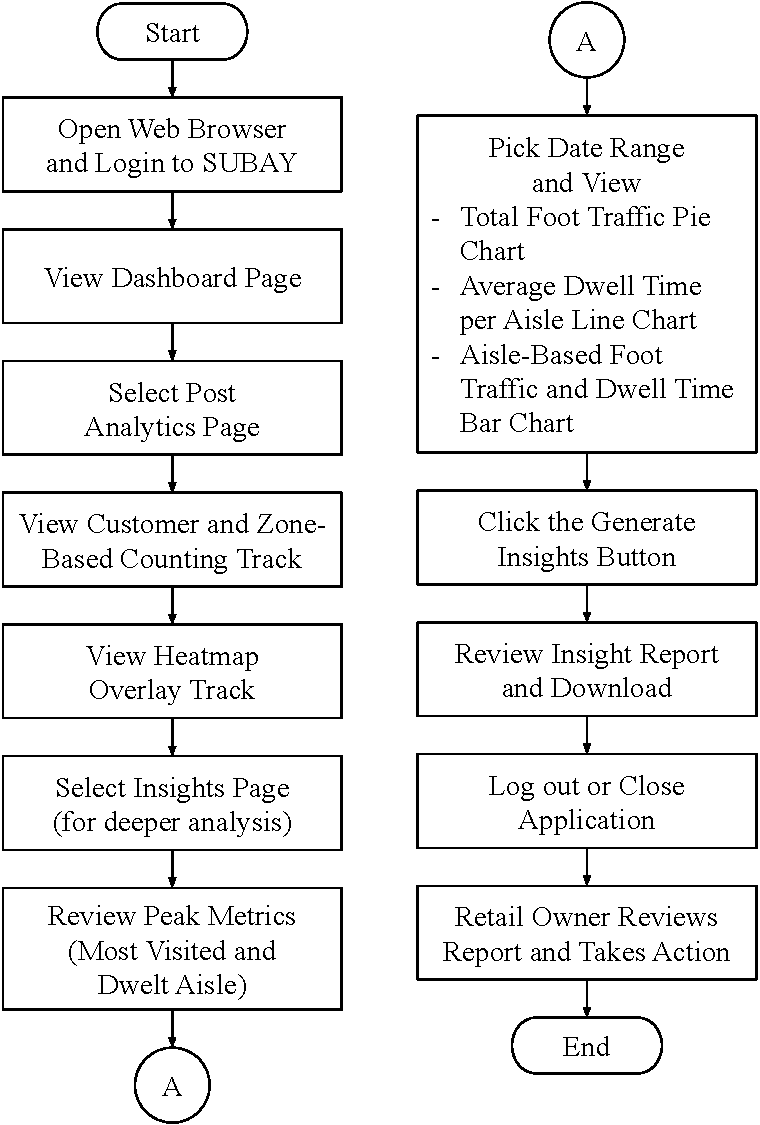
\includegraphics[width=0.40\linewidth]{fig/3.11.pdf}
	\label{fig:3.11}
\end{figure}

The activity diagram as shown on Figure~\ref{fig:3.11} illustrates the typical user flow for retail store owners or managers utilizing the SUBAY system. It begins with accessing the web application and navigating through the dashboard to the Post Analytics and Insights pages. Users can explore zone-based customer counts, heatmaps, and peak metrics such as the most visited and dwell aisles. The process continues with selecting a date range and generating charts that visualize total foot traffic, average dwell time, and zone-specific interactions. A detailed diagram for the insight generation phase will be presented to elaborate on this process. Finally, reports are reviewed and acted upon accordingly.

\begin{figure}[H]
	\caption[Insight Generation Activity Diagram]{\newline \newline Insight Generation Activity Diagram}
	\centering
	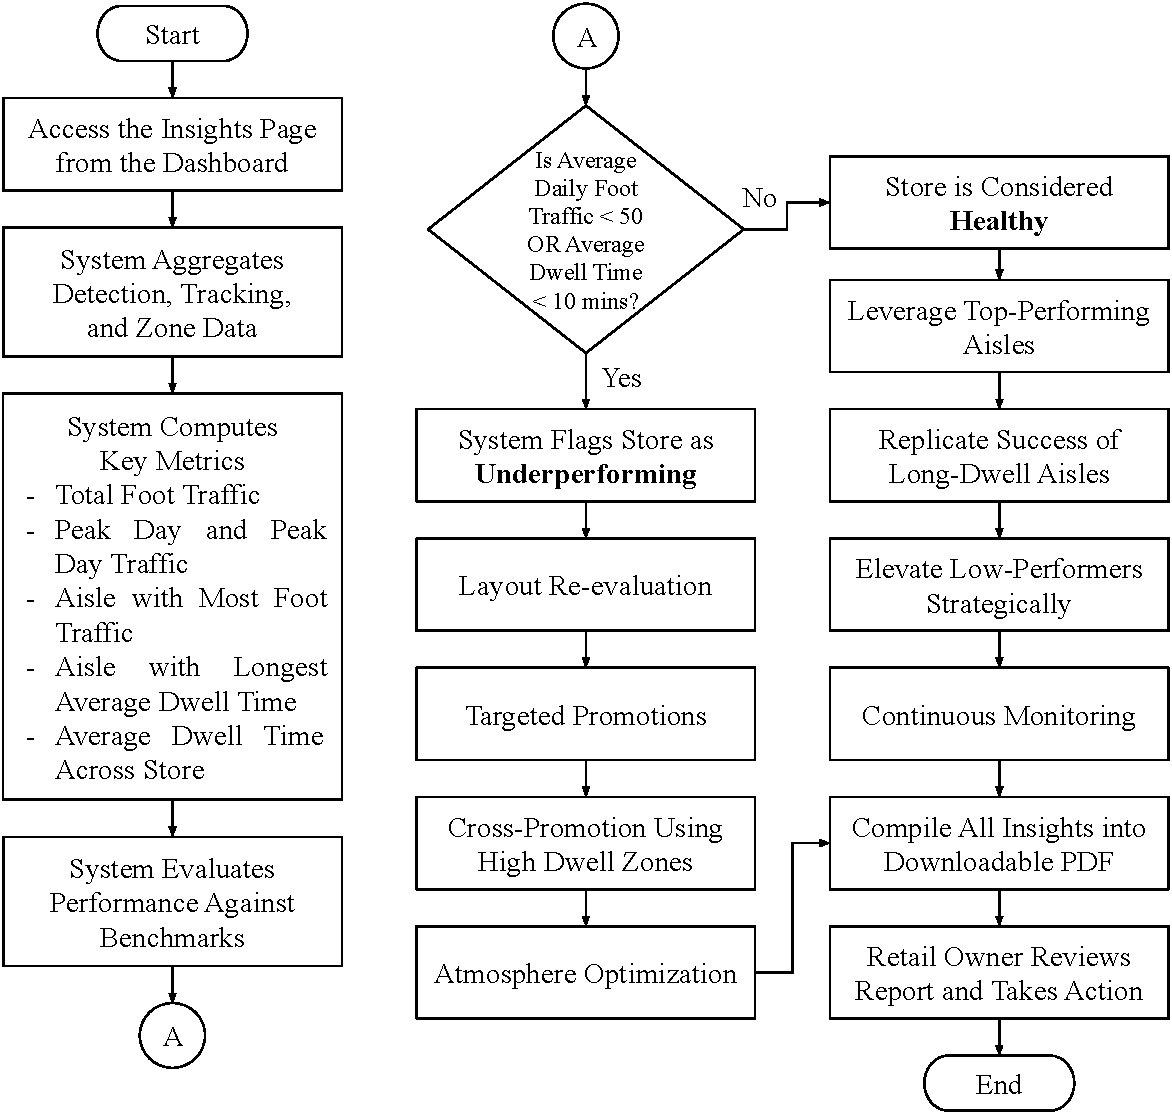
\includegraphics[width=0.80\linewidth]{fig/3.12.pdf}
	\label{fig:3.12}
\end{figure}

As shown in Figure~\ref{fig:3.12}, upon navigating the Insights Page, the system automatically processes all collected behavioral data from previous detection, tracking, and zone monitoring. Using the backend datasets, it computes essential performance metrics, including the total number of customer entries (foot traffic) during the monitored period, the peak day in terms of entries, zone-specific traffic volumes, average and peak dwell times, and the percentage breakdown of visits per zone. These metrics are evaluated against industry-aligned benchmarks: a daily average foot traffic threshold of 50 customers and an average dwell time of 10 minutes. These values were based on research from sources like \cite{BPlanAI2025} and \cite{CountTrack2025}, which identify underperformance in gift shops, especially those selling beauty and home products, when engagement or movement is below these thresholds.

\noindent\textbf{If the Store Is Flagged as Underperforming}

If averageDailyFootTraffic $<$ 50 or averageCustomerDwellTime $<$ 10 mins, the system concludes that the store is currently underperforming and automatically generates the following insights and actions based on the suggestions and recommendations in the articles by \cite{BPlanAI2025} and \cite{CountTrack2025}:

\textbf{Layout Re-evaluation:} The system suggests reassessing the spatial layout of underperforming aisles (e.g., Aisle C or D). The store manager may consider widening tight spaces, rearranging congested product racks, and improving line-of-sight to make items more visible and accessible. For instance, if Aisle C only had 5\% of the traffic, products might be moved closer to high-traffic intersections to boost exposure.

\textbf{Targeted Promotions:} Promotions such as discounts or bundle deals can be introduced in these low-traffic zones to encourage customer exploration. The system recommends prioritizing aisles with low visits and dwell time, suggesting that neither foot traffic nor customer interest is sustained in those sections.

\textbf{Cross-Promotion Using High Dwell Zones:} If Aisle A had the longest dwell time, the system recommends placing high-margin or complementary items (e.g., perfumes near hair care products) in that zone or its vicinity. Customers tend to linger where they’re intrigued, leveraging this zone to promote slower-moving products improves overall conversion.

\textbf{Atmosphere Optimization:} The system recommends better lighting, cleaner aisle signage, or even thematic decorations to attract attention. Aesthetic enhancements can invite customers into previously ignored areas.

\noindent\textbf{If the Store Is Performing Well}

If averageDailyFootTraffic $\geq$ 50 and averageCustomerDwellTime $\geq$ 10 minutes, the system concludes healthy engagement and provides insights to maintain or amplify success based on the suggestions and recommendations in the articles by \cite{BPlanAI2025} and \cite{CountTrack2025}:

\textbf{Leverage Top-Performing Aisles:} If Aisle B had 30\% of total foot traffic, placing promotional stands or new arrivals here could maximize reach and conversions. Popular aisles should act as marketing touchpoints.

\textbf{Replicate Success of Long-Dwell Aisles:} If Aisle A has a 40-minute average dwell time, the system recommends analyzing its product types, lighting, arrangement, and spacing. These characteristics can be mirrored in other aisles to boost performance.

\textbf{Elevate Low-Performers Strategically:} The system doesn’t ignore low-performing areas even if the store is healthy overall. Recommendations include mirroring top aisle attributes or rotating products to test customer response.

\textbf{Continuous Monitoring:} Managers are encouraged to monitor these metrics weekly, noting changes during promotional events, holidays, or layout changes. This supports evidence-based adjustments over time.

\subsubsection{System Architecture}
This section presents the system architecture. It illustrates the services, layers, components, architecture, and interactions and serves as the physical blueprint of the system.

Figure~\ref{fig:3.13} below illustrates the complete system architecture of SUBAY. The process begins with video footage captured from four strategically placed CCTV cameras. These video streams are processed through a detection module utilizing the YOLOv10 model, known for its high accuracy in detecting individuals. Following detection, the DeepSORT tracking algorithm maintains consistent tracking of individuals across multiple frames and camera views, enabling reliable mapping of customer movement throughout the store. The store layout is divided into predefined zones, allowing the system to focus behavioral analysis on specific areas. Movement patterns, zone occupancy, and customer flow are systematically captured and analyzed.

A heat mapping module further enriches this analysis by visualizing dwell time and movement intensity, using color gradients to highlight areas of high customer engagement. All collected behavioral data, including foot traffic metrics, zone visits, dwell time, and heat map visuals, are transmitted to an analytics dashboard. 

\begin{figure}[H]
\	\caption[System Architecture]{\newline \newline System Architecture}
	\centering
	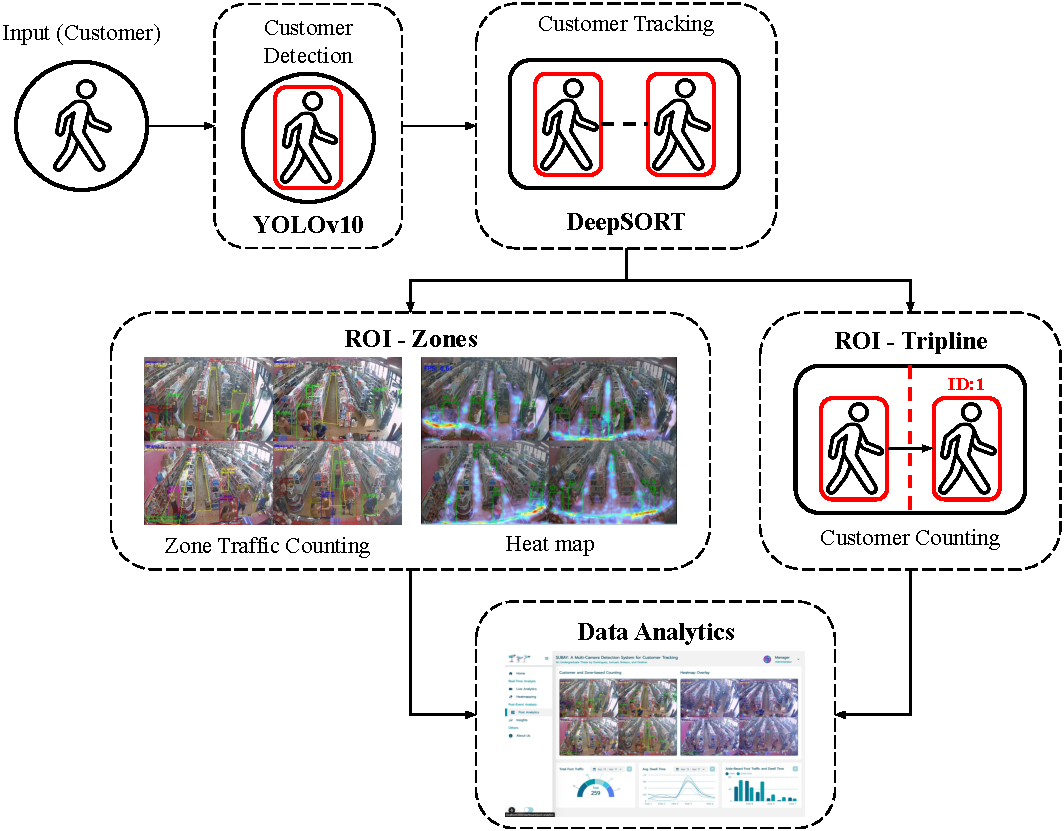
\includegraphics[width=1\linewidth]{fig/3.13.pdf}
	\label{fig:3.13}
\end{figure}

This dashboard serves as the primary interface for retail managers, presenting data in user-friendly visual formats. Managers can monitor foot traffic trends through the dashboard, evaluate zone effectiveness, and gain deeper insights into customer behaviors. These insights support strategic decisions on store layout optimization and product placement, ultimately boosting their sales performance.

\subsection{Implementation}

The implementation phase focused on developing the software components of the SUBAY system, leveraging the store’s existing CCTV infrastructure as the primary video input source. This minimized setup complexity and facilitated seamless integration into the retail environment.

\begin{figure}[H]
	\caption[Steps in Implementing SUBAY]{\newline \newline Steps in Implementing SUBAY}
	\centering
	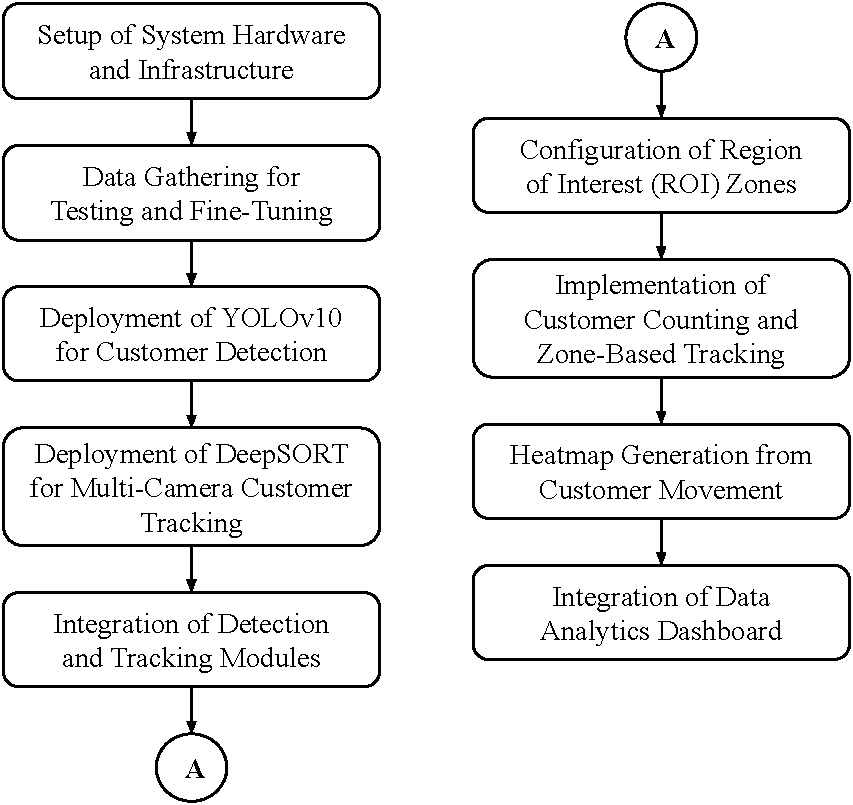
\includegraphics[width=0.50\linewidth]{fig/3.14.pdf}
	\label{fig:3.14}
\end{figure}

As illustrated in Figure~\ref{fig:3.14}, the implementation began by configuring a high-performance computing (HPC) unit designed to handle the computational demands of real-time video processing. The system followed a structured pipeline: customer detection, tracking, re-identification, zone monitoring, and behavioral data aggregation. The first stage involved deploying YOLOv10, a deep learning object detection model, to accurately localize individuals within each video frame captured from multiple cameras. Detected customers were then passed to DeepSORT, an advanced tracking algorithm, to assign and maintain unique identities as they moved across camera views. DeepSORT was enhanced with OSNet, a person re-identification model that preserved identity consistency even under occlusion, lighting changes, and camera transitions for added robustness.

Regions of Interest (ROIs) were manually defined across strategic areas such as aisles and product shelves to enable zone-based analytics. The system continuously monitored customer presence within these zones, calculated dwell time, and generated active customer counts based on the assigned tracking IDs. These behavioral metrics were visualized through heat maps using color gradients to represent spatial engagement and movement density. All outputs, including customer counts, zone engagement, dwell time, and heat maps, were integrated into the SUBAY analytics dashboard. This dashboard served as the final interface for retail managers, offering an intuitive view of customer behavior to support layout optimization and data-driven promotional strategies.

The development environment employed two primary configurations: Microsoft Visual Studio Code IDE for structured Python code development and debugging, and a Linux-based HPC text editor for resource-efficiently executing training scripts and video processing pipelines. The system was built on a robust and modular software stack. Python served as the primary development language, with PyTorch used for deep learning operations, TorchReID for re-identification, and OpenCV and NumPy for computer vision and numerical processing. The motion prediction and data association tasks were handled using the Kalman Filter and the Hungarian Algorithm. Visual outputs such as heat maps were refined for clarity using Gaussian-based rendering, alpha blending, and morphological operations.

To achieve high-speed processing and reliable performance, the system utilized CUDA-enabled GPU acceleration and multithreaded execution through ThreadPoolExecutor and Threading. Tracking accuracy was further improved through Cosine Similarity and Intersection over Union (IoU) metrics. YAML configuration files were used to streamline model and system parameter settings. This implementation strategy enabled SUBAY to process video feeds, track customers accurately across multiple views, and generate actionable behavioral analytics with speed, precision, and efficiency.

\subsubsection{Customer Detection}

The implementation of customer detection in this study centered on deploying a convolutional neural network (CNN)-based object detection model, You Only Look Once version 10 (YOLOv10). YOLOv10 served as the foundation of the system’s detection pipeline, identifying customers from video input captured by four pre-installed CCTV cameras positioned at store entrances, aisles, and display zones. This setup provided continuous coverage without requiring additional hardware installation.

Video feeds were processed frame by frame, where YOLOv10 generated bounding boxes, class labels, and confidence scores to detect and localize individuals. These outputs allowed the system to highlight customers’ positions within each frame while filtering out non-customer objects and background noise.

To improve detection performance under real-world conditions, the model was periodically fine-tuned using additional footage from the store itself. This incremental training allowed the system to adapt to variations in lighting, customer appearance, and crowd density, ensuring consistent detection accuracy.

\begin{figure}[H]
	\caption[The Architecture of YOLO CNN \citep{Artamonov2018}]{\newline \newline The Architecture of YOLO CNN \citep{Artamonov2018}}
	\centering
	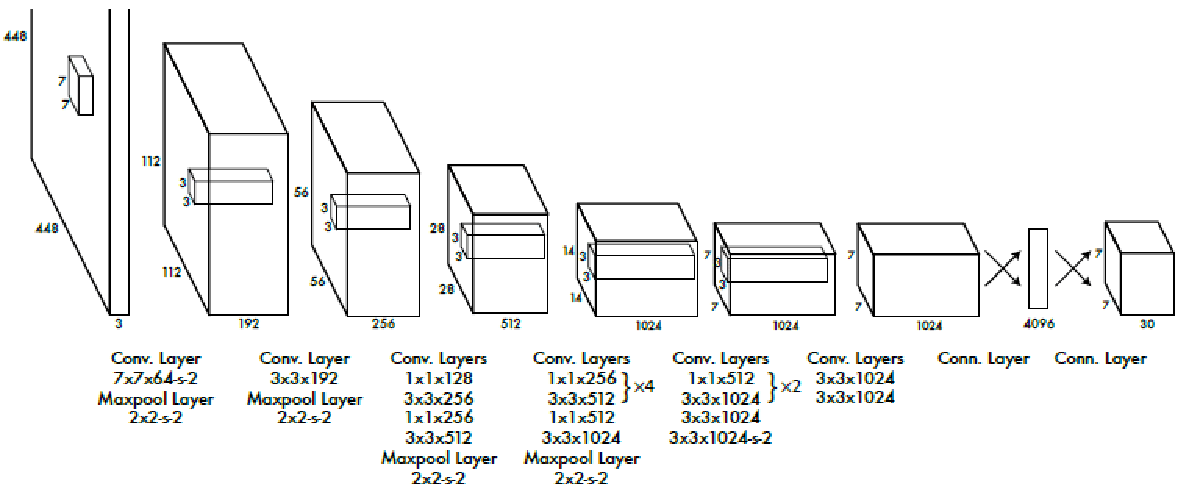
\includegraphics[width=1\linewidth]{fig/3.15.pdf}
	\label{fig:3.15}
\end{figure}

As shown in Figure~\ref{fig:3.15}, the detection process started with YOLOv10 extracting spatial features from each frame through a series of convolutional layers. The detected individuals were then passed to the tracking module, where they were assigned persistent IDs for continuous monitoring across frames and cameras. This seamless flow between detection and tracking enabled reliable zone monitoring, heat mapping, and analytics generation.

Figure~\ref{fig:3.16} outlines the customer classification process used in the system. Video streams were broken into frames and analyzed to detect entities such as shelves, carts, and people, each labeled with a confidence score. An object filtering stage was applied to remove false positives based on size, movement, and location criteria. Detections showing human-like movement and features were classified as customers.

\begin{figure}[H]
	\caption[Classifying Customers Diagram]{\newline \newline Classifying Customers Diagram}
	\centering
	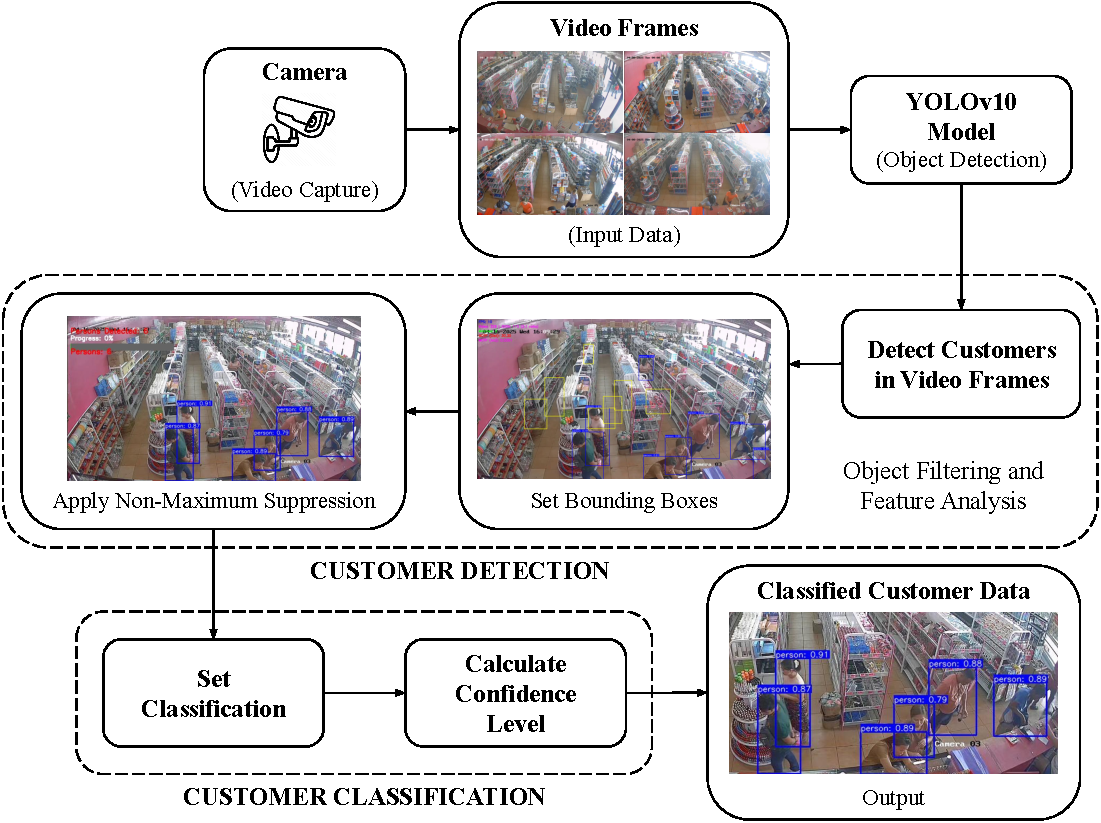
\includegraphics[width=0.75\linewidth]{fig/3.16.pdf}
	\label{fig:3.16}
\end{figure}

A confidence scoring module evaluated detection reliability by considering motion patterns, object shape, and clarity. Verified customers were then assigned a unique ID, spatial coordinates, and a classification confidence score. Only these structured, high-confidence detections were passed to downstream modules for tracking, counting, zone analysis, and heat map generation, ensuring the system’s outputs remained accurate and actionable.

\subsubsection{Customer Tracking}

To maintain persistent identification of customers throughout their in-store journey, the system combined YOLOv10 for object detection with DeepSORT for object tracking. This integration allowed accurate monitoring of individuals across frames, even when partial occlusion, camera switching, or brief disappearances occurred.

While YOLOv10 localized customers in single frames, it could not associate their identities over time. DeepSORT addressed this by introducing a deep Re-Identification (Re-ID) model, which extracted appearance features from each detected individual. These features matched identities across frames, reducing ID-switching and ensuring consistent tracking.

\begin{figure}[H]
	\caption[DeepSORT: SORT with a Deep Association Metric \citep{Admin2023}]{\newline \newline DeepSORT: SORT with a Deep Association Metric \citep{Admin2023}}
	\centering
	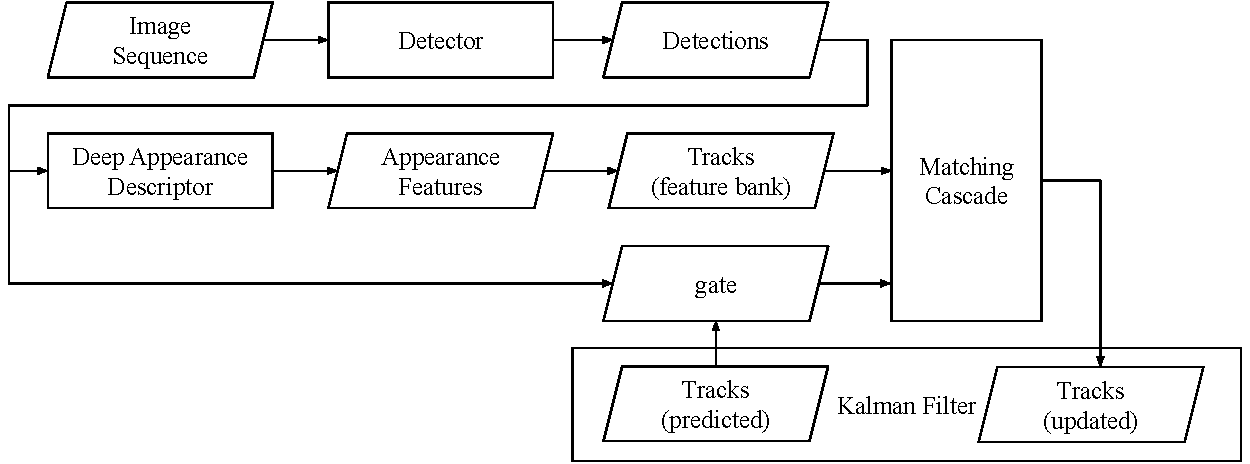
\includegraphics[width=0.75\linewidth]{fig/3.17.pdf}
	\label{fig:3.17}
\end{figure}

As shown in Figure~\ref{fig:3.17}, detection outputs from YOLOv10 were passed through a feature extractor to generate appearance vectors. These vectors were compared with existing tracked identities using a matching cascade based on appearance similarity and motion predictions. A Kalman filter refined the estimated locations, integrating new detection data with past movement patterns to maintain stable and smooth trajectories.

Figure~\ref{fig:3.18} below illustrates the assignment and maintenance of unique customer IDs. Upon detection, individuals were given a persistent ID consistent across frames and camera views. If a visual match was found based on features like color, shape, and motion, the ID and trajectory were updated; otherwise, a new ID was assigned. This process prevented duplication and maintained accurate tracking continuity.

\begin{figure}[H]
	\caption[Tracking Customer IDs]{\newline \newline Tracking Customer IDs}
	\centering
	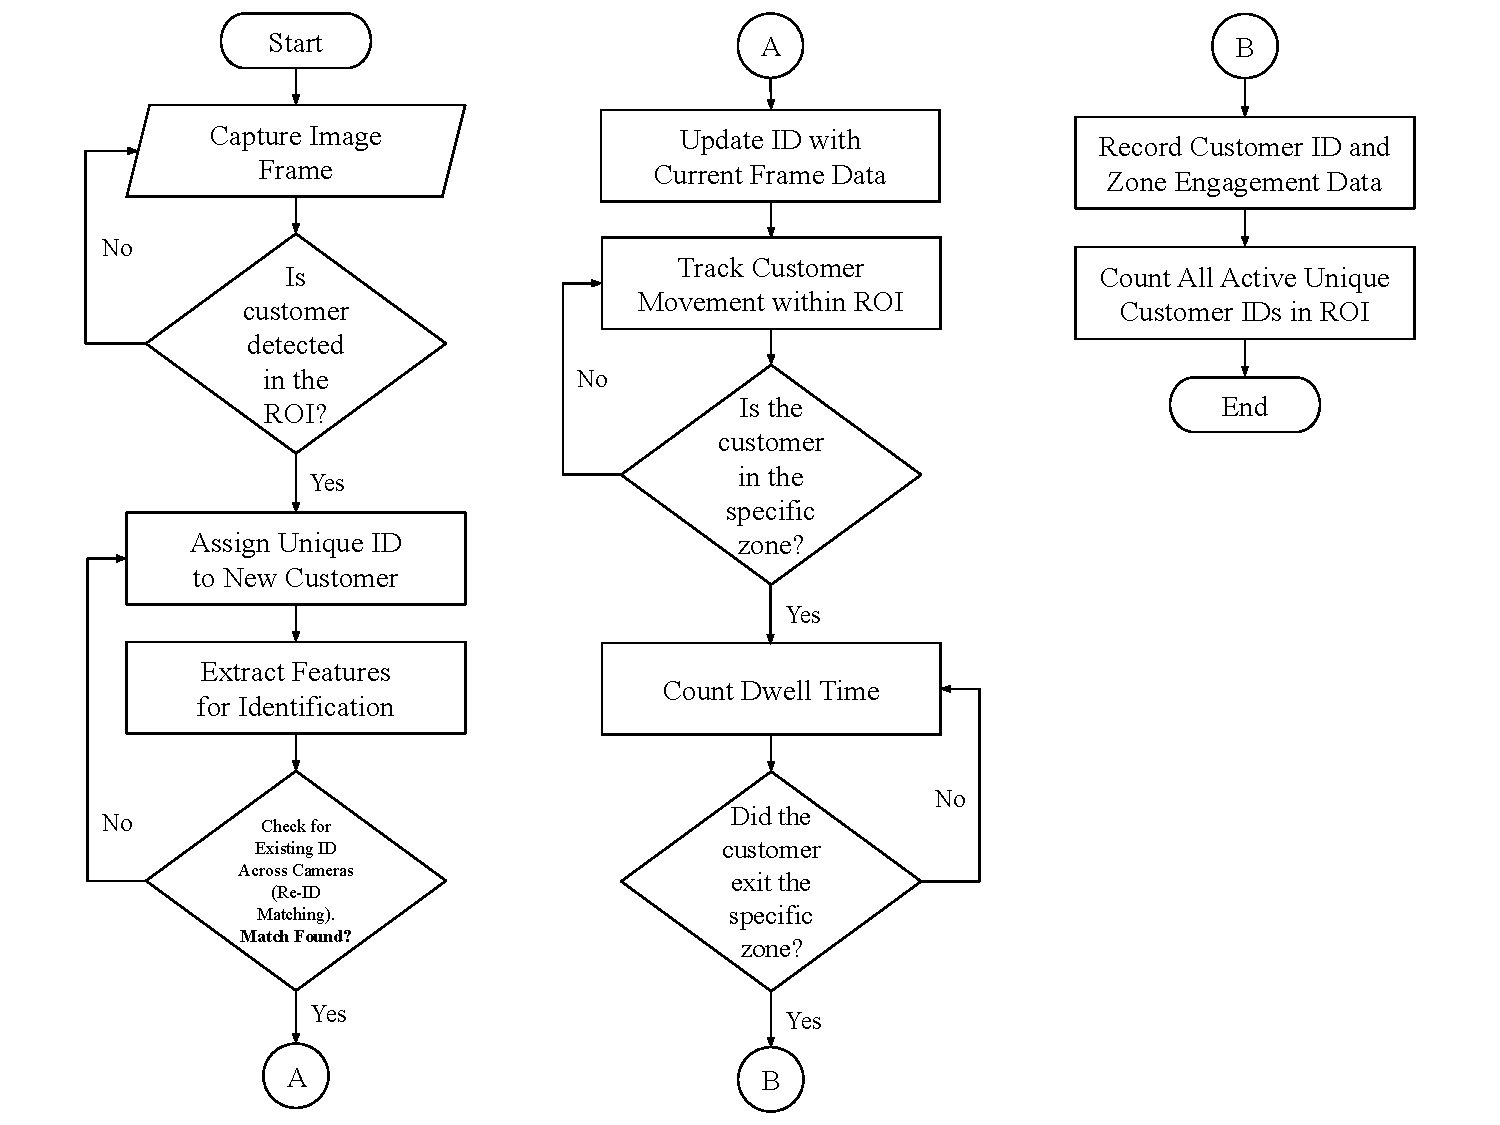
\includegraphics[width=1\linewidth]{figs/3.18.pdf}
	\label{fig:3.18}
\end{figure}

DeepSORT is effective for tracking individuals within a single camera stream; however, it struggles to maintain consistent identity tracking across multiple camera frames, especially when individuals move between non-overlapping fields of view. The system integrated OSNet (Omni-Scale Network) into the DeepSORT pipeline to overcome this limitation and improve person re-identification (Re-ID) across cameras. OSNet enhances identity recognition by capturing fine-grained and global appearance features through multiple convolutional streams within a single residual block. As illustrated in Figure~\ref{fig:3.19}, its unified aggregation gate adaptively prioritizes relevant features, improving robustness to occlusion, pose variation, and lighting differences.

\begin{figure}[H]
	\caption[A Schematic of the Proposed Building Block for OSNet. R: Receptive field size. \citep{Boujou2022}]{\newline \newline A Schematic of the Proposed Building Block for OSNet. R: Receptive field size. \citep{Boujou2022}}
	\centering
	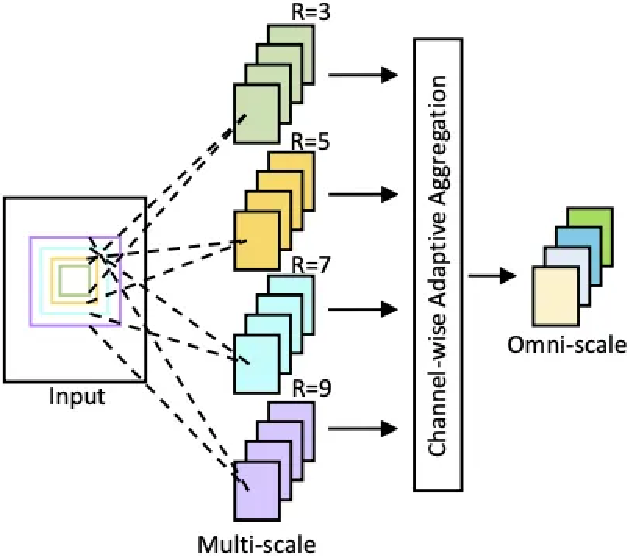
\includegraphics[width=0.50\linewidth]{fig/3.19}
	\label{fig:3.19}
\end{figure}

Despite its detailed feature extraction, OSNet remained computationally efficient, making it ideal for retail applications. By leveraging OSNet, the system achieved consistent identity matching across different camera angles and challenging conditions. As customers moved through predefined Regions of Interest (ROIs), the system tracked entries, dwell times, and movement paths. These tracking records were later used to generate zone engagement metrics and behavioral flow analysis, supporting data-driven retail decision-making.

\subsubsection{Customer Counting}

The SUBAY system combined object detection with multi-object tracking to accurately measure foot traffic, moving beyond traditional tripline-only methods. Instead of relying solely on fixed lines, it used intelligent detection and tracking across multiple camera views to prevent redundant or missed counts.

As shown in Figure~\ref{fig:3.20}, the process began with video streams from the store’s CCTV cameras. YOLOv10 detected individuals frame by frame, while DeepSORT tracked them across multiple frames and angles. A Region of Interest (ROI) tripline was placed at a key entrance view to identify new customer entries.

\begin{figure}[H]
	\caption[Customer Counting Process]{\newline \newline Customer Counting Process}
	\centering
	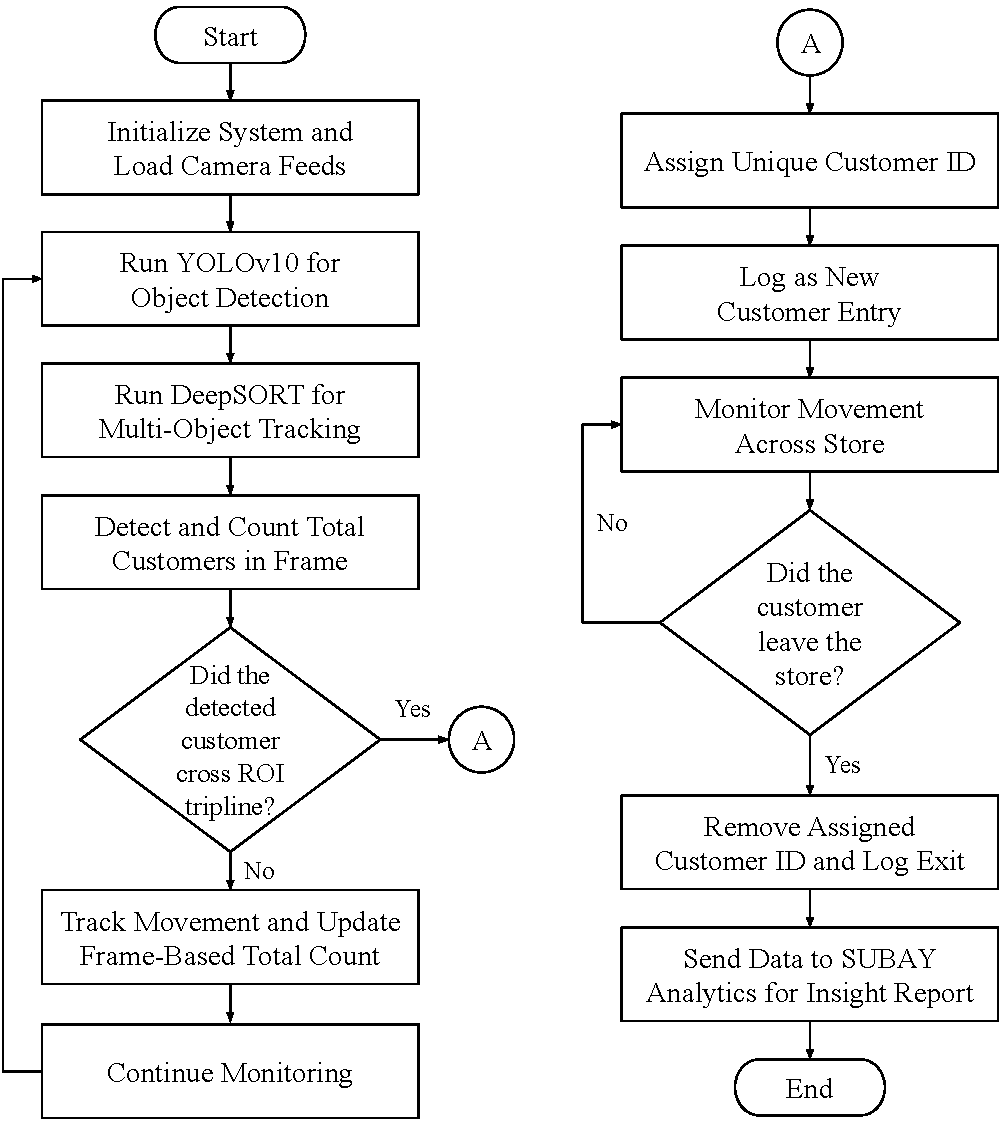
\includegraphics[width=0.50\linewidth]{fig/3.20.pdf}
	\label{fig:3.20}
\end{figure}

When a detected individual crossed the tripline in the correct direction, the system logged the event as a new entry and assigned a unique ID for tracking. This ID remained active while the customer stayed inside and was discarded upon exit. The system maintained reliable, non-redundant entry counts by combining continuous frame-based monitoring with directional tripline detection. All collected counting data, including current presence and cumulative foot traffic, was forwarded to the SUBAY analytics dashboard to support operational insights and store performance evaluation.

The system maintained reliable, non-redundant entry counts by combining continuous frame-based monitoring with directional tripline detection. All collected counting data, including current presence and cumulative foot traffic, was forwarded to the SUBAY analytics dashboard to support operational insights and store performance evaluation.

\subsubsection{Zoning and Heat Mapping}

The SUBAY system implemented zone monitoring based on predefined Regions of Interest (ROIs) to better understand how customers interacted with specific areas. These zones were mapped onto camera views covering important retail spaces like aisles and product displays.

\begin{figure}[H]
	\caption[Customer Counting Inside Zone Process]{\newline \newline Customer Counting Inside Zone Process}
	\centering
	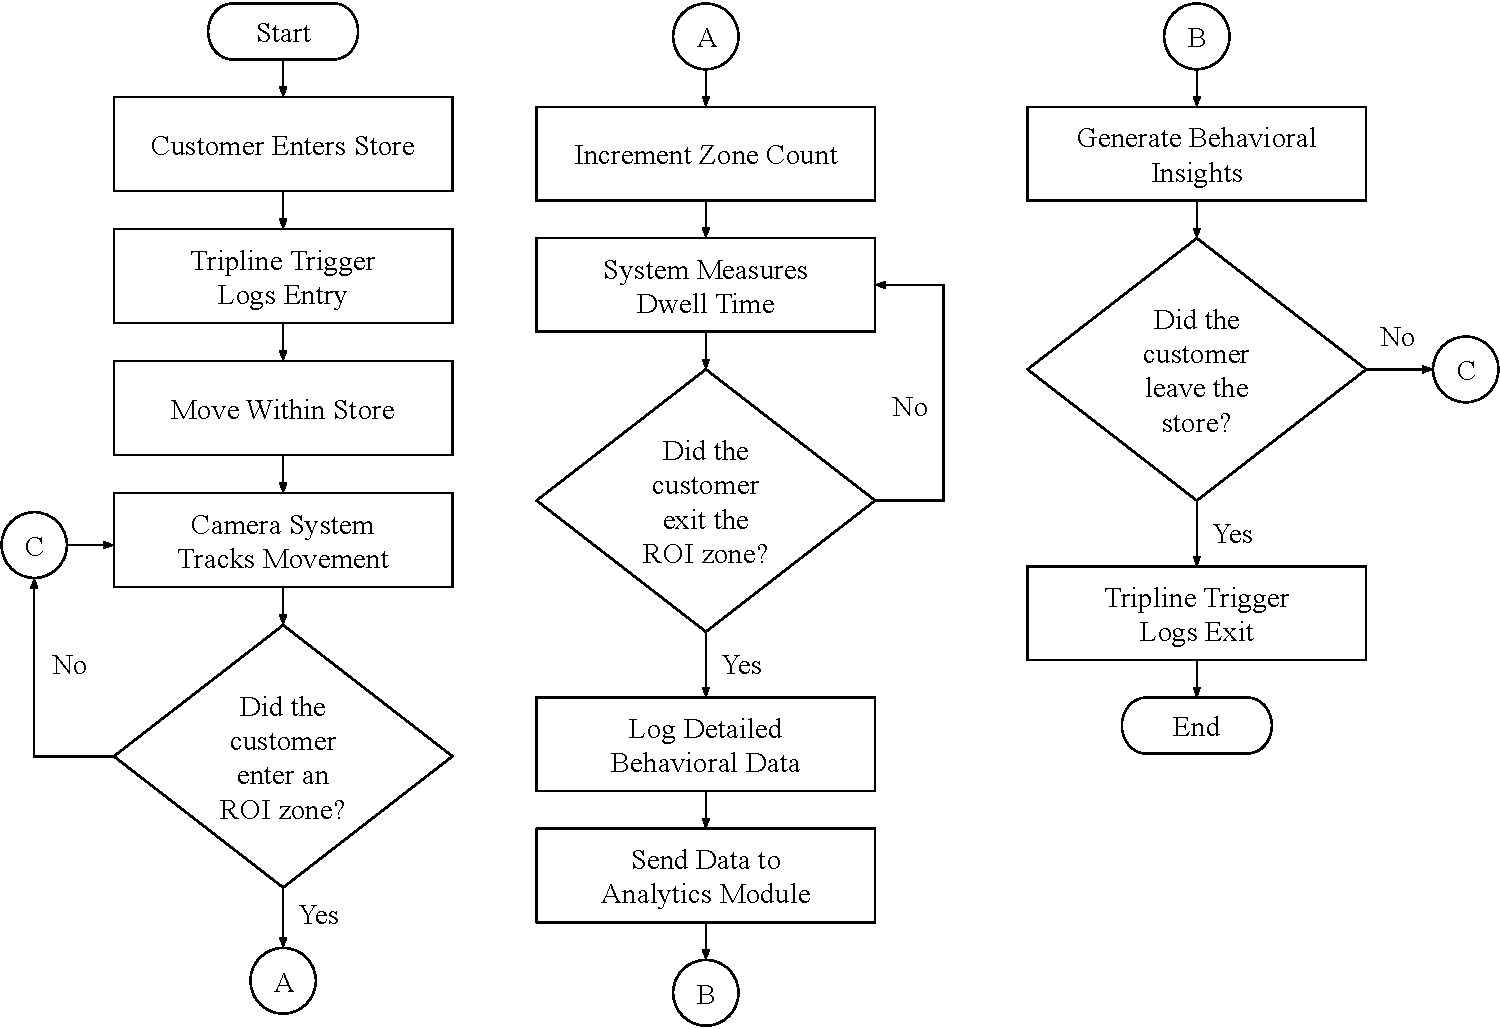
\includegraphics[width=0.75\linewidth]{fig/3.21.pdf}
	\label{fig:3.21}
\end{figure}

As shown in Figure~\ref{fig:3.21}, the system is initialized by connecting to the store’s CCTV cameras, which provide overlapping coverage to minimize blind spots. Once live, YOLOv10 detected individuals in each frame while DeepSORT maintained their unique IDs across angles and occlusions. When a customer entered an ROI, the system triggered a dwell time counter and incremented the zone’s traffic count. This movement data was stored for later analysis and formed the basis for behavioral insights and heat map generation.

\begin{figure}[H]
	\caption[Heat Map Generation Process]{\newline \newline Heat Map Generation Process}
	\centering
	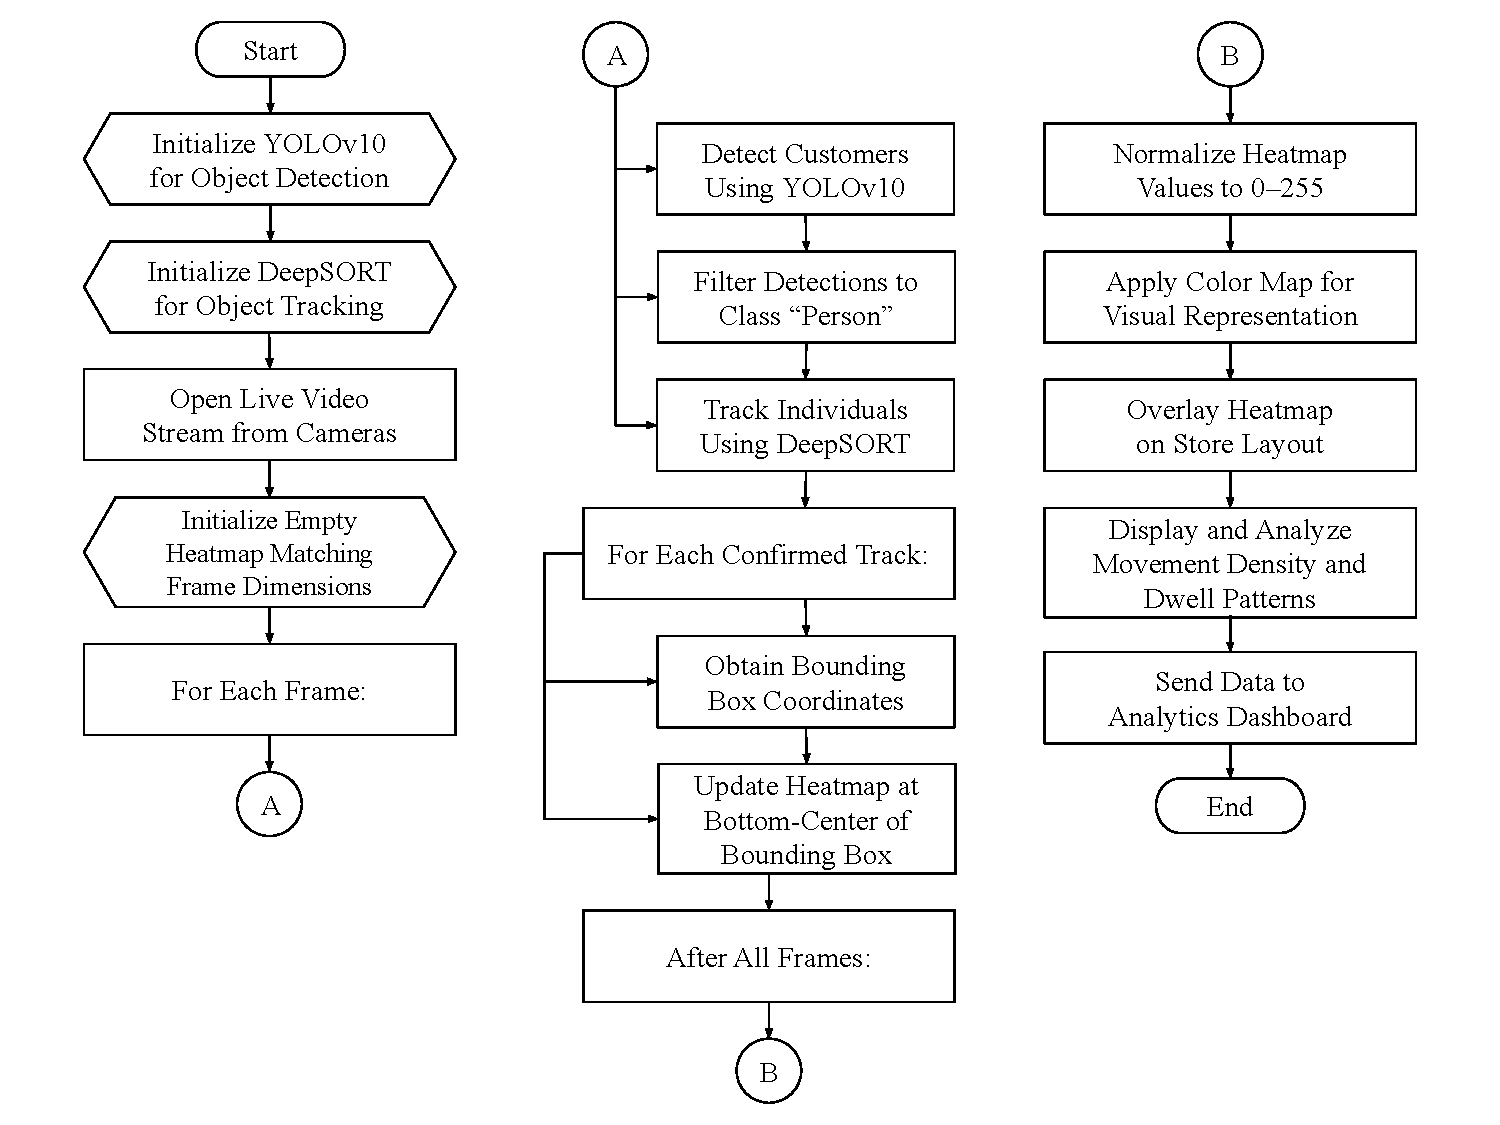
\includegraphics[width=1\linewidth]{figs/3.22.pdf}
	\label{fig:3.22}
\end{figure}

Figure~\ref{fig:3.22} shows how heat maps were created. As video frames were processed, YOLOv10 and DeepSORT tracked each customer's position, marking the bottom-center of their bounding box to map movement within the store. These incremental location updates built a density map, visually representing foot traffic intensity over time. Once processed, the heat map values were normalized, colorized using a gradient, and overlaid on the store layout.

This allowed managers to quickly spot high-engagement areas and underutilized spaces, supporting layout adjustments and marketing strategies. The resulting heat maps and zone metrics were forwarded to the SUBAY dashboard for straightforward interpretation and decision-making.

\subsubsection{Customer Analytics}

The customer behavior analytics module in the SUBAY system was designed to extract actionable insights from tracked movement and interactions within the retail environment. This module operated by capturing surveillance footage from multiple cameras and applying computer vision techniques to interpret customer behavior, specifically, how individuals moved through the store, where they lingered, and which products or zones drew their attention.

As shown in Figure~\ref{fig:3.23}, the system followed a streamlined pipeline that began with detection and tracking using YOLOv10 and DeepSORT. These models ensured consistent identification of individuals across overlapping camera zones, minimizing blind spots and maintaining reliable trajectories. Aggregated movement data, such as zone entries, dwell durations, and path continuity, were then analyzed to produce behavioral metrics.

To inform the final system's user interface and navigation structure, the researchers began by designing the web application using Figma. Wireframes and low-fidelity prototypes were created to map out the application's layout and user flow. This design phase allowed for early visualization of the platform’s core features, including analytics dashboards, navigation menus, and data filters. Iterative refinements were made based on usability and feedback, ensuring that the final system would be accessible and intuitive for retail users with varying technical backgrounds.

\begin{figure}[H]
	\caption[Customer Analytics Process]{\newline \newline Customer Analytics Process}
	\centering
	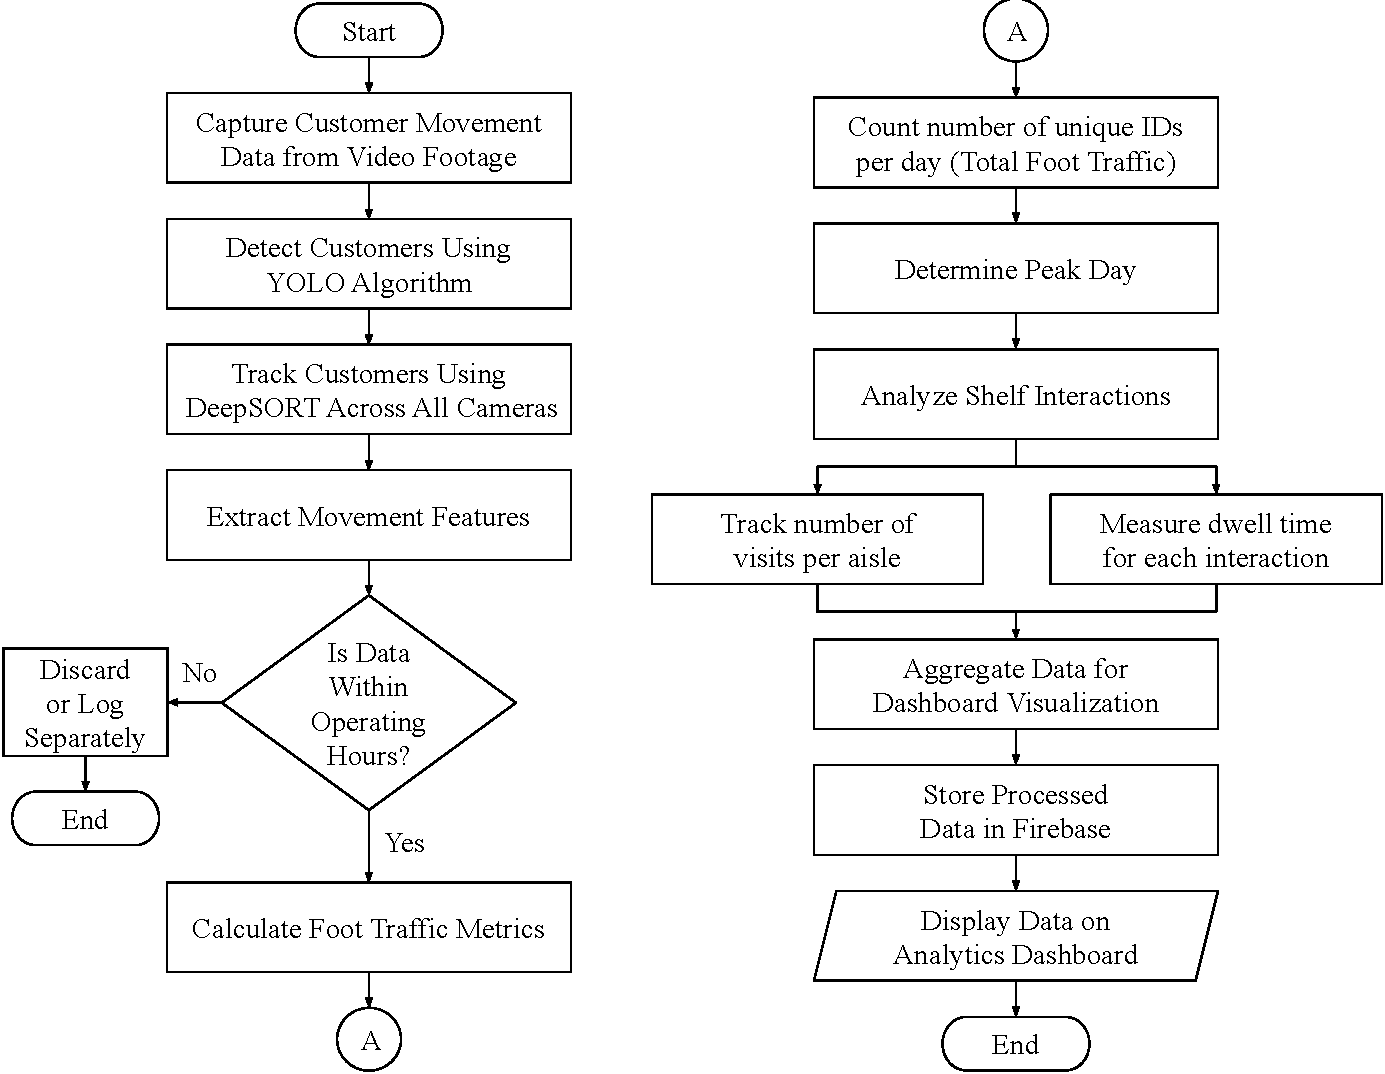
\includegraphics[width=1\linewidth]{fig/3.23.pdf}
	\label{fig:3.23}
\end{figure}

After finalizing the interface design, the researchers implemented the SUBAY web application using modern development technologies. Next.js 15 with TypeScript was used for core application logic, while Tailwind CSS provided a utility-first framework for responsive and customizable styling. ReactJS enabled dynamic, component-based front-end development, enhancing the system’s interactivity and performance. Firebase Cloud Firestore is a real-time NoSQL database on the backend for scalable data storage and retrieval. GitHub was used for version control, supporting collaborative development and secure tracking of code changes. The entire system architecture operated within a Node.js environment, ensuring reliability and responsiveness.

The detection and tracking data collected from video feeds were filtered to exclude activity outside of store hours, maintaining the integrity of the analytics. The system generated key behavioral indicators from this curated data, such as aisle visitation frequency, zone-specific dwell times, heatmap intensity, and peak activity periods.

These insights were visualized through an analytics dashboard that provided interactive charts, graphs, and summary cards. Retail managers could explore metrics such as total daily foot traffic, dwell time distributions, and customer interaction patterns across different store sections. This allowed them to make informed, data-driven decisions about store layout, product placement, and marketing strategy.

Although Live Analytics and Heatmap Overlay pages were also developed to demonstrate the system’s real-time monitoring capabilities, they were excluded from the final deployed version. As outlined in the study’s scope and limitations, only Post-Event Analysis features were retained for deployment. These features allowed the store owner to review and reflect on customer behavior after it occurred, offering valuable insights while preserving system simplicity and privacy. The SUBAY system effectively transformed raw surveillance footage into structured behavioral insights through a robust pipeline of detection, tracking, and analytics delivered via a web application designed to be both functional and user-friendly.

\subsection{Testing \& Evaluation}

To ensure that the SUBAY system met its intended requirements, it underwent a thorough testing and evaluation process. These activities involved the researchers and the intended end user, the retail store owner, to identify any defects, performance issues, or usability concerns that could impact the system’s reliability in a real-world retail environment.

\subsubsection{Testing}

The system was subjected to several levels of testing to verify its functionality and compliance with design specifications. Unit testing was first conducted to validate the performance of individual modules, including camera integration, object detection using YOLO, customer tracking via DeepSORT, and the analytics dashboard. Each module was tested independently to ensure it functioned correctly.

Following this, integration testing evaluated how well the modules worked together, focusing on the seamless data transfer between the detection, tracking, and dashboard components. System testing was then performed to assess the integrated system's operation under real-world conditions, such as customer movement and varying lighting scenarios.

Finally, user acceptance testing (UAT) was conducted with the retail store owner. During this phase, users performed typical tasks while the system’s behavior and their feedback were observed. UAT confirmed the system’s readiness in terms of usability, effectiveness, and alignment with the users’ operational needs.

\subsubsection{Evaluation}

The evaluation process involved both functional and usability testing. A black-box approach was used for functional testing, where different input scenarios were applied without examining the system's internal structure. A customized testing form based on the project’s requirement specifications was used to record whether the system’s outputs aligned with the intended behaviors.

The System Usability Scale (SUS) developed by \cite{Brooke1995} was employed for usability testing. Participants were guided through major system features, such as viewing camera feeds, tracking customer movement, and accessing analytics. Afterward, they completed the SUS questionnaire to assess the system's ease of use, learnability, and user satisfaction. The results provided a quantifiable measure of how intuitive and user-friendly the system was for retail staff. This structured evaluation process refined the SUBAY system to meet technical and end-user expectations, ensuring its readiness for deployment.

\subsubsection{Evaluating Multi-Object Tracking Accuracy and Performance Metrics}

A detailed evaluation of its multi-object tracking performance was conducted to further validate the SUBAY system’s ability to monitor customer movement. The assessment focused on detection accuracy, identity preservation, and tracking precision, using key performance metrics drawn from \cite{Li2023} shown in Table 3.3.

\begin{longtable}[H]{|c|>{\centering\arraybackslash}m{2.2cm}|>{\centering\arraybackslash}m{6.2cm}|>{\centering\arraybackslash}m{3.8cm}|}
	\caption[Evaluation Indicators for Multi-Object Tracking \citep{Li2023}]{\newline \newline Evaluation Indicators for Multi-Object Tracking \citep{Li2023}}\label{tab:mot_metrics}\\
	\hline
	\textbf{Eqn No.} & \textbf{Metric} & \textbf{Formula} & \textbf{Description} \\
	\hline
	\endfirsthead
	
	\multicolumn{4}{c}%
	{\tablename\ \thetable\ -- \textit{Continued from previous page}} \\
	\hline
	\textbf{Eqn \#} & \textbf{Metric} & \textbf{Formula} & \textbf{Description} \\
	\hline
	\endhead
	
	\hline \multicolumn{4}{r}{\textit{Continued on next page}} \\
	\endfoot
	
	\hline
	\endlastfoot
	
	3.1
	& Multiple Object Tracking Accuracy (MOTA) 
	& 
	$
	\text{MOTA} = 1 - \frac{\sum_{t}(FN_t + FP_t + ID\_Swt)}{\sum{t}GT_t}$
	Where:
	\begin{itemize}
		\item $FN_t$: False Negatives at time $t$
		\item $FP_t$: False positives at time $t$
		\item $ID_Sw_t$: ID Switches at time $t$
		\item $GT_t$: Ground Truth Objects at time $t$
	\end{itemize}
	& MOTA was used to measure the overall accuracy of the tracking system by accounting for false positives, false negatives, and ID switches during tracking \citep{Fei2023}. This metric helped determine how well the system avoided tracking errors in practical deployment. \\
	\hline
	
	3.2 
	& Multiple Object Tracking Precision (MOTP) 
	& 
	$
	\text{MOTP} = \frac{\sum{i_t}d{i_t}}{\sum_{t}c_t}
	$
	\newline
	\newline
	Where:
	\begin{itemize}
		\item $d_t$ = 1 - \textit{IOU}, the distance between the ground truth and predicted bounding boxes for object \textit{i} in frame $t$.
		\item $c_t$, the number of matches in frame $t$.
	\end{itemize}
	& MOTP measured how precisely the system localized and tracked individuals. It was calculated based on the Intersection over Union (IoU) of bounding boxes between detected objects and ground truth. This formula measures the average localization precision across all correctly matched pairs in the video sequence \citep{Fei2023}. This metric indicated the system’s spatial tracking precision within the store layout. \\
	\hline
	3.3 
	& Identification Precision (IDP) 
	& $\text{IDP} = \frac{IDTP}{IDTP + IDFP}$
	\newline
	\newline
	Where IDTP and IDFP are the number of valid and false positive IDs, respectively, a high IDP score indicates that customer identities were not incorrectly assigned or merged.
	& IDP evaluated how accurately the system identified and maintained customer identities during tracking. Simply, it is the accuracy of customer ID identification in each bounding box \citep{Fei2023}. \\
	\hline
	3.4 
	& Identification Recall (IDR) 
	& 
	$\text{IDR} = \frac{IDTP}{IDTP + IDFN'}$
	\newline
	\newline
	Where IDFN is the negative ID number, this ensured that the system consistently detected and retained the identities of all customers entering or moving within camera range.
	& IDR assessed how well the system captured and maintained all customer identities across frames. It is the recall rate of customer ID identification in each bounding box \citep{Fei2023}. \\
	\hline
	3.5 
	& Identification F1 Score (IDF1) 
	& 
	$
	\text{IDF1} = \frac{2 \times IDP \times IDR}{IDP + IDR}
	$
	\newline
	\newline
	This metric reflected the system's effectiveness in maintaining consistent identity tracking across multiple frames and camera views.
	& IDF1 represented the harmonic mean between IDP and IDR, offering a balanced measure of identification accuracy. It is the F-value of the customer ID in each bounding box \citep{Fei2023}.\\
\end{longtable}

These tracking performance metrics confirmed that the SUBAY system could reliably track and analyze customer movement patterns even under challenging retail conditions. The results from this evaluation were used to optimize the detection thresholds and improve the synchronization between detection and tracking modules, ultimately contributing to more accurate behavioral analytics and better retail decision-making.

}